\section{Continuum mechanics}

Continuum mechanics allows to define general equations of motion for a wide range of phenomena from liquids to deformable solids. 
In this section, we propose a progressive introduction to the basics of continuum mechanics and provide details about the physical models used in the following chapters. 
Firstly, we describe how to formulate general equations of motion and we present the different concepts and numerical tools used to solve them.
Secondly, we present a constitutive law for fluid mechanics leading to Navier-Stokes equations and we detail their discretization using the Smoothed-Particle Hydrodynamics (SPH) model that will serve as background for our contribution in Chapter~\ref{chap:arps}.
Finally, we present a constitutive law for solid mechanics which allows to simulate elastic solids and we detail the discretization of the equations of motion using the frame-based model that we use in Chapter~\ref{chap:cutting}.
If the reader looks for a wider presentation of the existing deformable models in Computer Graphics, we suggest the survey of Nealen et al.~\cite{Nealen2006}.
%\subsection{Notation}
%
%We will use the following notations throughout this manuscript.
%\begin{table}[!h]
%\begin{tabular}{ll}
%$t$ & time \\
%$m$ &  mass \\
%$\rho$ & mass density \\
%$\mathbf{n}$ & normal \\
%$\mathbf{x}$ & position \\
%$\mathbf{v}$ & velocity \\
%$\mathbf{f}$ & total forces \\
%$\mathbf{f}_{int}$ & internal forces \\
%$\mathbf{f}_{ext}$ & external forces \\
%$F$ & Deformation gradient \\
%$\epsilon$ & Strain tensor \\
%$\sigma$ & Stress tensor \\
%$\Psi$ & Energy density \\
%\end{tabular}
%\end{table}
\subsection{Equations of motion}
\label{subsec:starMechanics_motionEquation}
The equations of motion describe the behavior of an object over time.
They are generally derived from conservation laws such as mass and momentum conservation. 
A constitutive law is also used to depict the intrinsic behavior of the simulated object.
The remainder of this section first describes the conservation laws used to formulate general equations of motion.
Then we detail the concepts and numerical tools used to solve these equations.

\subsubsection{Conservation of mass}
\label{subsubsec:starMechanics_massConservation}
The conservation of mass states that, whatever the physical material which is studied, mass cannot be created or destroyed.
More precisely, if we look at a small volume of the simulation domain, the variation of mass in that volume should be equal to the flux of mass going through its border.
In Figure~\ref{fig:massConservation}, we illustrate this law with the example of a glass of water.
At a time $t_{1}$, the mass of the water should be equal to its mass at time $t_{0}$ plus the mass of the inflow and minus the mass of the outflow which occurred between $t_{0}$ and $t_{1}$.
\begin{figure}[!h]
	\centering
	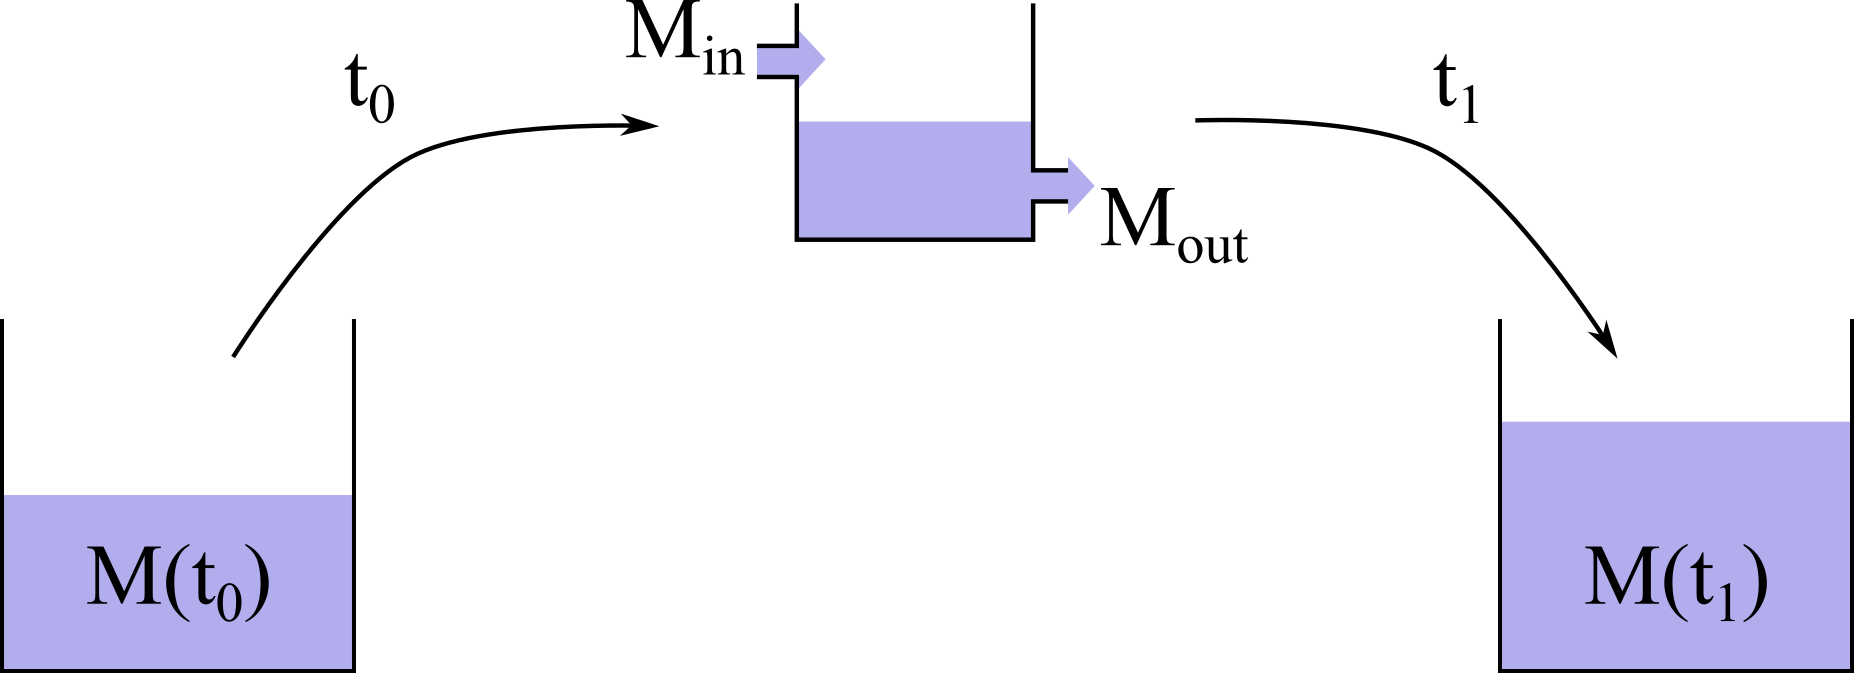
\includegraphics[width=\linewidth]{images/continuum_mechanics/massConservation.png}
	\caption[STAR mechanics: Mass conservation]{\label{fig:massConservation} Mass conservation. $M(t_{1}) = M(t_{0}) + M_{in} - M_{out}$}
\end{figure}
\\
Mathematically, we can write the conservation of mass as
\begin{equation}
    \label{eq:massConservation}
    \displaystyle 
    \frac{d}{dt}\left( \int_{\mathcal{V}} \rho(t,\mathbf{x}) dv \right)
    =
    - \int_{\mathcal{\partial V}}\rho(t,\mathbf{x})\mathbf{v}(t,\mathbf{x}) \cdot \mathbf{n}(\mathbf{x}) ds
\end{equation}
where
\begin{itemize}
	\item $\rho(t,\mathbf{x})$ is the density at a point $\mathbf{x}$ and at a time $t$.
	\item $\mathbf{v}(t,\mathbf{x})$ is the velocity at a point $\mathbf{x}$ and at a time $t$.
	\item $\mathcal{V}$ is a small volume of the simulation domain $\Omega$.
	\item $\mathcal{\partial V}$ is the border of $\mathcal{V}$.
	\item $\mathbf{n}(\mathbf{x})$ is the normal outward of $\mathcal{V}$ on a point $\mathbf{x}$ of $\partial\mathcal{V}$.
\end{itemize}
This formulation involves an integral over the volume and its boundary.
When numerically solving this equation, it is simpler not to have to make the distinction between a small element of $\mathcal{V}$ and a small element of $\partial \mathcal{V}$.
By using Stokes' theorem, we have
\begin{equation}
\displaystyle 
\int_{\partial \mathcal{V}} \rho \mathbf{v} \cdot \mathbf{n} ds =
\int_{\mathcal{V}} \nabla \cdot \left( \rho \mathbf{v} \right) dv
\end{equation}
and we can rewrite Equation~\eqref{eq:massConservation} as a single integral over $\mathcal{V}$
\begin{equation}
\label{eq:volumetricMassConservation}
\displaystyle 
\int_{\mathcal{V}} 
\left( \frac{\partial \rho}{\partial t} + \nabla \cdot \left( \rho  \mathbf{v} \right) \right) dv = \mathbf{0}
\end{equation}

\subsubsection{Conservation of momentum}
\label{subsubsec:starMechanics_momentumConservation}
The conservation of momentum is implied by Newton's second law which states that the forces applied on an object result into an acceleration which is inversely proportional to the mass of the object.
Figure~\ref{fig:momentumConservation} illustrates this law in the case of two balls on which a same force is applied.
The acceleration induced by the force is more important for the small ball which has a mass less important than the big ball.
\begin{figure}[!h]
\centering
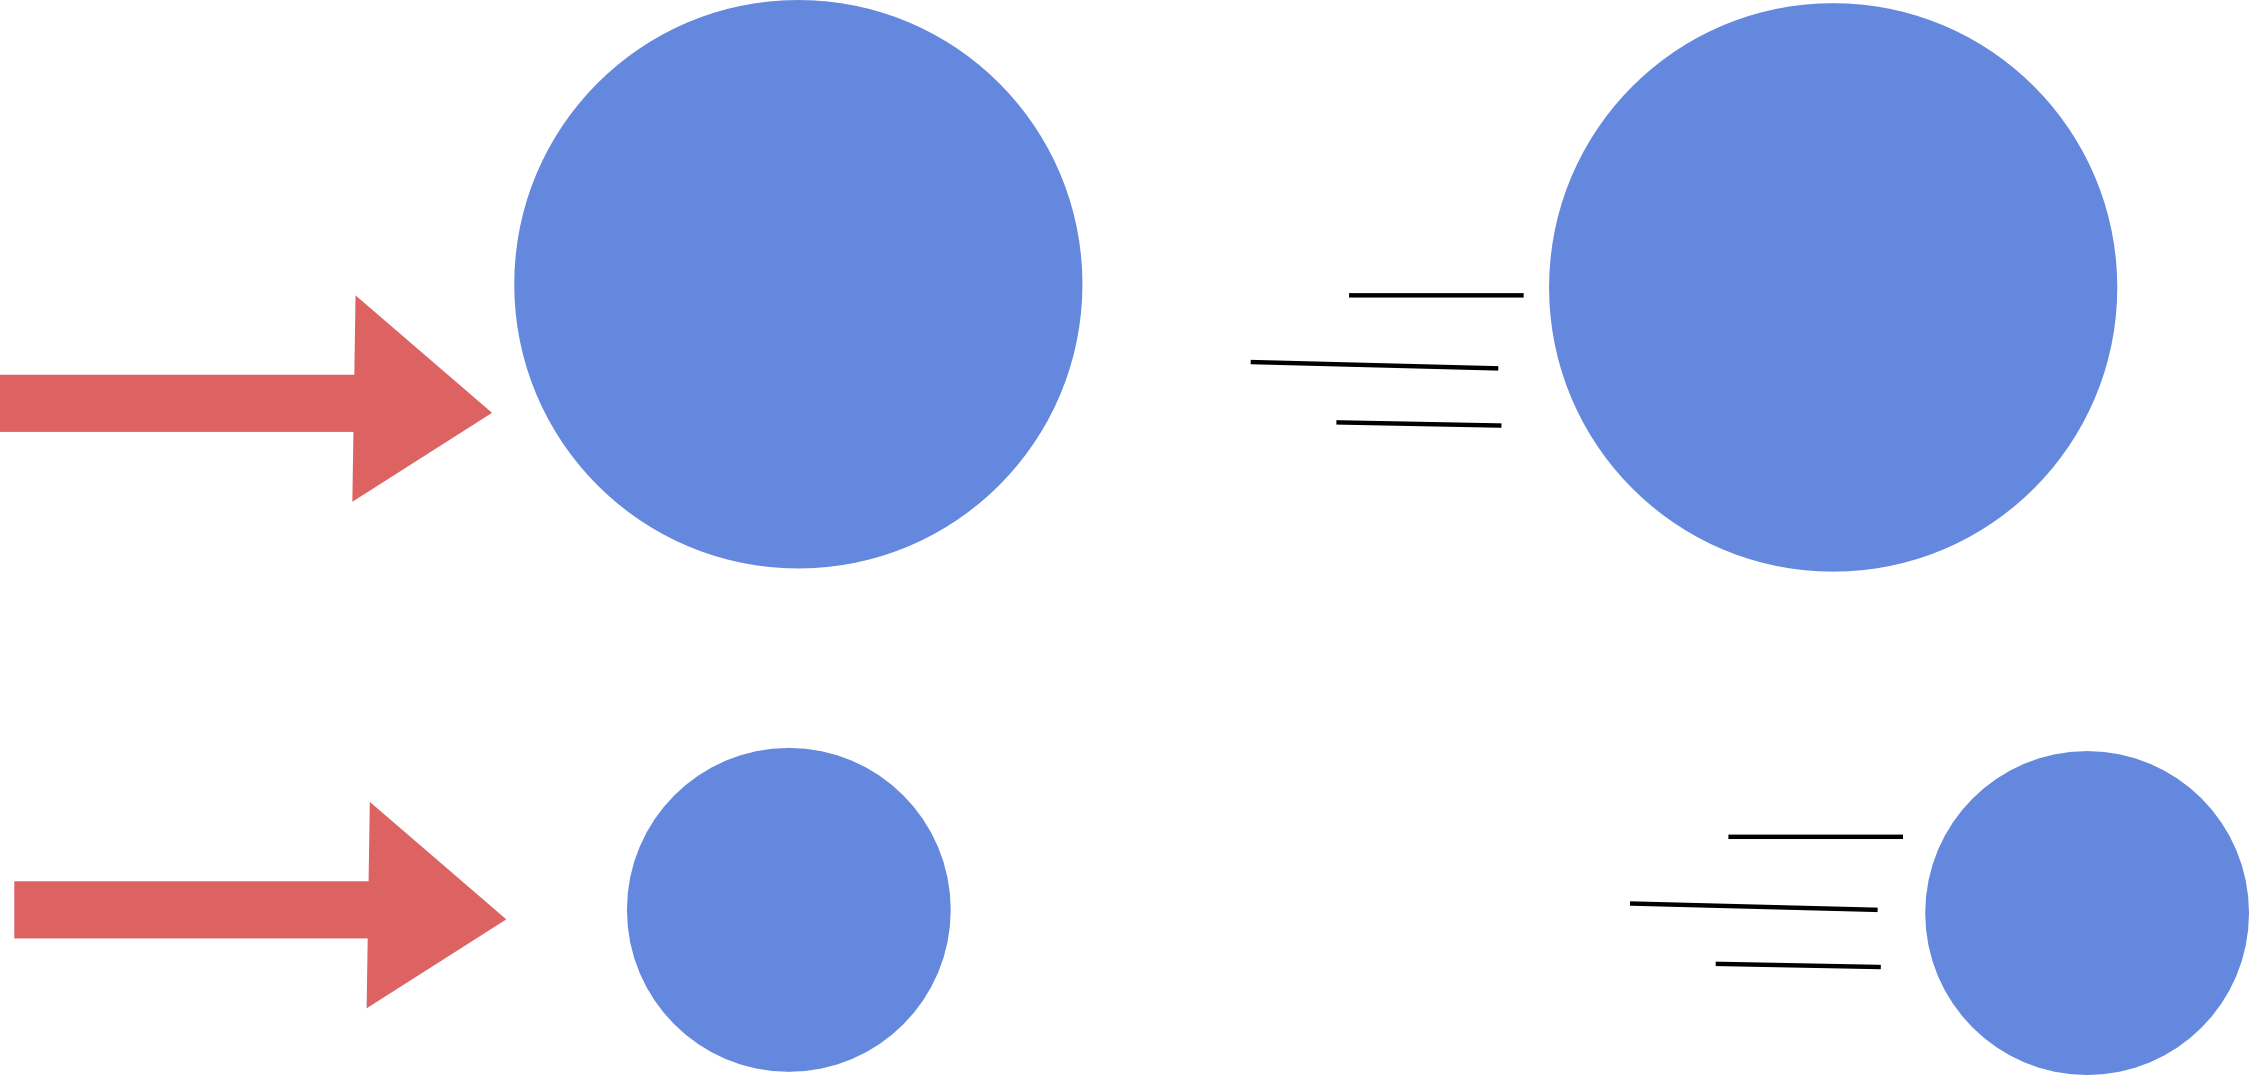
\includegraphics[width=\linewidth]{images/continuum_mechanics/momentumConservation.png}
\caption[STAR mechanics: Momentum conservation]{\label{fig:momentumConservation} Momentum conservation. The same force $\mathbf{f}$ is applied on two balls. The resulting acceleration is inversely proportional to their mass.}
\end{figure}
\\
Mathematically, this law can be written as
\begin{equation}
\displaystyle 
\int_{\mathcal{V}} 
\rho(t,\mathbf{x})\mathbf{a}(t,\mathbf{x}) dv 
= 
\int_{\mathcal{V}} \mathbf{f}(t,\mathbf{x}) dv
\end{equation}
where
\begin{itemize}
	\item $\mathbf{a}(t,\mathbf{x})$ is the acceleration at a point $\mathbf{x}$ and at a time $t$.
		\item $\mathbf{f}(t,\mathbf{x})$ is the force applied on a point $\mathbf{x}$ and at a time $t$.
\end{itemize}
By performing a Taylor-Young expansion on the acceleration, we can re-write the momentum conservation as
\begin{equation}
\label{eq:momentumConservation}
\displaystyle 
\int_{\mathcal{V}} 
\rho(t,\mathbf{x}) \left( \frac{\partial\mathbf{v}}{\partial t} + \mathbf{v} \cdot \nabla \mathbf{v} \right)(t,\mathbf{x}) dv 
= 
\int_{\mathcal{V}} \mathbf{f}(t,\mathbf{x}) dv
\end{equation}
Two kind of forces are generally applied on an object, the \emph{external} forces and the \emph{internal} forces.
External forces describe the action of the surrounding environment on the object. 
The simplest example is the weight, i.e. the force applied by the constant gravity $\mathbf{g}$ on the object:
\begin{equation}
\label{eq:externalForces}
\displaystyle \int_{\mathcal{V}} \mathbf{f}_{ext}(t,\mathbf{x})dv = \int_{\mathcal{V}} \rho(t,\mathbf{x}) \mathbf{g} dv
\end{equation}
Internal forces describe the reaction of the object to an external deformation.
Generally, they are defined by using a stress tensor $\sigma(t,\mathbf{x})$ as 
\begin{equation}
\displaystyle 
\int_{\mathcal{V}} \mathbf{f}_{int}(t,\mathbf{x}) dv 
= \int_{\partial \mathcal{V}} \sigma(t,\mathbf{x}) \mathbf{n}(\mathbf{x}) ds
\end{equation}
Basically, the stress relates the deformation of the object to its material properties by using a constitutive law.
A constitutive law is specific to the phenomena which is simulated.
In Section~\ref{subsec:fluidMechanics} and Section~\ref{subsec:solidMechanics}, we will respectively describe the most common constitutive laws for incompressible fluids and solids.
For a detailed and intuitive definition of the stress tensor we refer the reader to the \emph{SIGGRAPH} course about real-time physics~\cite{Muller2008} by M\"{u}ller et al.
\\
Same as for the conservation of mass, we can use Stokes' theorem to get a single integral over $\mathcal{V}$,
\begin{equation}
\label{eq:internalForces}
\displaystyle 
\int_{\mathcal{V}} \mathbf{f}_{int}\left(t,\mathbf{x}\right) dv 
\int_{\mathcal{V}} \nabla \cdot \sigma\left(t,\mathbf{x}\right) dv
\end{equation}
and we can rewrite Equation~\eqref{eq:momentumConservation} as
\begin{equation}
\label{eq:volumetricMomentumConservation}
\displaystyle
\int_{\mathcal{V}} 
\left( 
\rho \left( \frac{\partial\mathbf{v}}{\partial t} + \mathbf{v} \cdot \nabla \mathbf{v} \right)
- \nabla \cdot \sigma - \rho \mathbf{g}  \right) dv = \mathbf{0}
\end{equation}

\subsubsection{Eulerian vs. Lagrangian formulations}
\label{subsubsec:starMechanics_eulerianLagrangian}
Eulerian and Lagrangian formulations are two different ways of interpreting the equations of motion.
To understand the key difference, we take the example of the simulation of a river and use Figure~\ref{fig:EulerianVsLagrangian} to illustrate it.
Let us suppose that we want to measure fluid properties such as velocity, density or temperature of the river.
A first possibility would be to measure it at a fixed location, similarly to a buoy that would remain at the same spot and measures data at regular intervals of time. This is the Eulerian viewpoint. A second possibility is to measure it along a path that would follow the flow of the river, similarly to an object floating on the river or a particle of water moving accordingly to the flow. This is the Lagrangian viewpoint.
\begin{figure}[!ht]
	\centering
	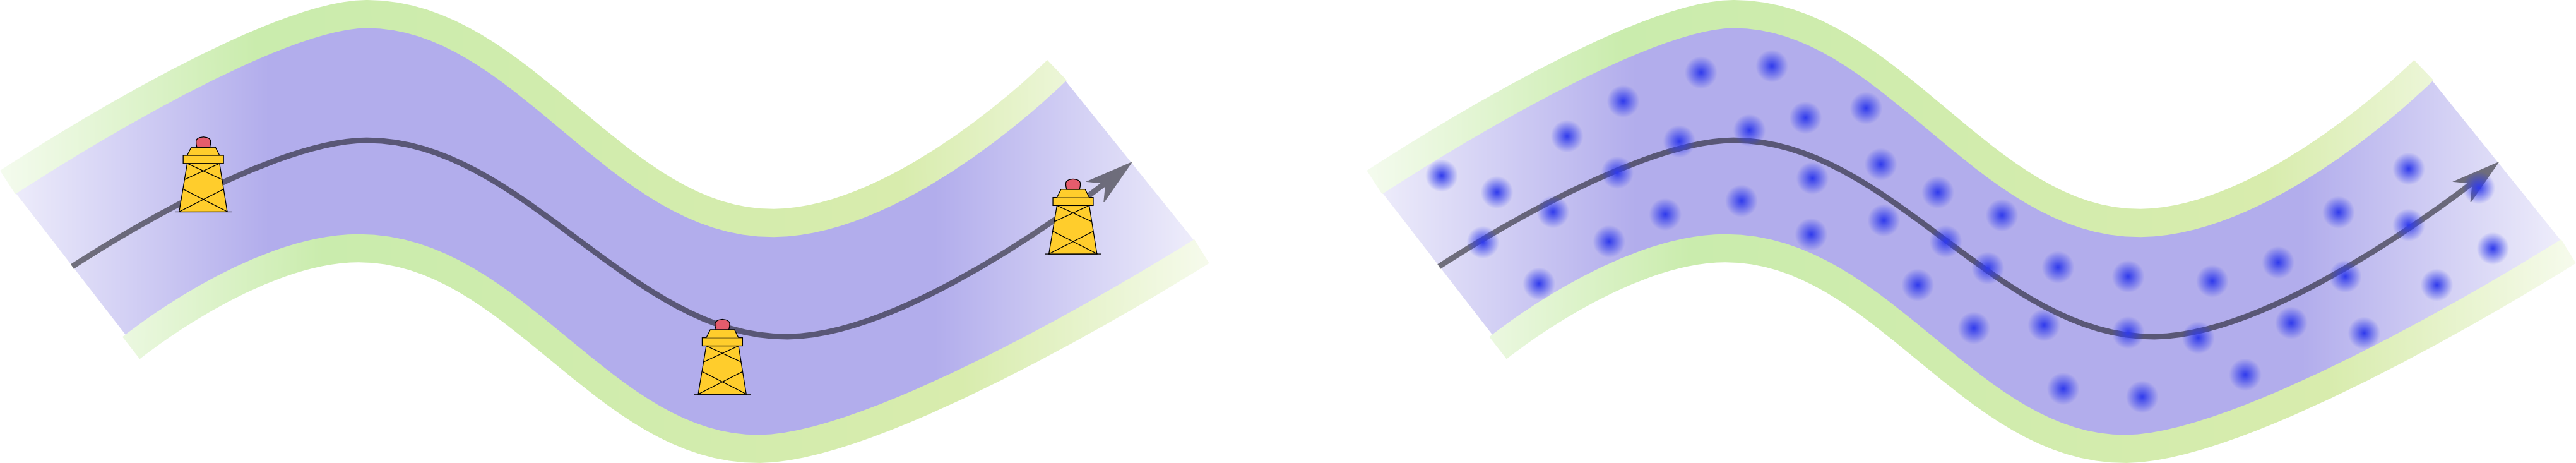
\includegraphics[width=\linewidth]{images/continuum_mechanics/eulerianVsLagrangian.png}
	\caption[STAR mechanics: Eulerian vs. Lagrangian]{\label{fig:EulerianVsLagrangian} Eulerian vs. Lagrangian viewpoint. On the left, buoys are put at fixed positions on a river and measure properties such as velocity, temperature, etc. The Eulerian approach takes a similar approach. On the right, we represent the river with particles of water which follows the flow of the river and carry properties with them. This is similar to the Lagrangian viewpoint.}
\end{figure}
Equation~\eqref{eq:volumetricMassConservation} and Equation~\eqref{eq:volumetricMomentumConservation} are described for fixed locations. Put together, they define the equations of motion from an Eulerian viewpoint.
\begin{equation}
\label{eq:eulerianMotionEquation}
\left\lbrace
\begin{array}{l}
\displaystyle 
\int_{\mathcal{V}} 
\left( 
\rho \left( \frac{\partial\mathbf{v}}{\partial t} + \mathbf{v} \cdot \nabla \mathbf{v} \right)
- \nabla \cdot \sigma - \rho \mathbf{g}  \right) dv = \mathbf{0}
\\ \\
\displaystyle
\int_{\mathcal{V}} 
\left( \frac{\partial \rho}{\partial t} + \nabla \cdot \left( \rho  \mathbf{v} \right) \right) dv = 0
\end{array}
\right.
\end{equation}
In order to adopt the Lagrangian viewpoint, let us suppose that the fluid properties are carried by particles and that $q(t,\mathbf{x})$ denote one of this property at a time $t$ for a particle which is at a position $\mathbf{x}$. 
If we want to compute the derivative of $q$ for the particle at position $\mathbf{x}$, we have to use the total derivative:
\begin{equation}
\label{eq:totalDerivative}
\frac{dq(t,\mathbf{x})}{dt} = 
\frac{\partial q}{\partial t}\cdot\frac{dt}{dt} + \frac{\partial q}{\partial \mathbf{x}} \cdot \frac{d\mathbf{x}}{dt} 
= \frac{\partial q}{\partial t}(t,\mathbf{x}) + \left(\nabla q(t,\mathbf{x}) \cdot \mathbf{v}\right)(t,\mathbf{x})
\end{equation}
In Equation~\eqref{eq:volumetricMomentumConservation} which describes the momentum conservation, we can directly use Equation~\eqref{eq:totalDerivative} to adopt a Lagrangian viewpoint. 
For the mass conservation described in Equation~\eqref{eq:volumetricMassConservation}, we first need to develop the divergence of the product between density and velocity and then Equation~\eqref{eq:totalDerivative} can be used.
Finally, we can write the equations of motion from a Lagrangian viewpoint as
\begin{equation}
\label{eq:lagrangianMotionEquation}
\left\lbrace
\begin{array}{l}
\displaystyle 
\int_{\mathcal{V}} 
\left( 
\rho \frac{d\mathbf{v}}{dt}
- \nabla \cdot \sigma - \rho \mathbf{g}  \right) dv = \mathbf{0}
\\ \\
\displaystyle
\int_{\mathcal{V}} 
\left( \frac{d\rho}{dt} + \rho \nabla \cdot \mathbf{v} \right) dv = 0
\end{array}
\right.
\end{equation}
As the deformable models used in Chapter~\ref{chap:arps} and Chapter~\ref{chap:cutting} are used to solve Lagrangian equations of motion, we will keep Equation~\eqref{eq:lagrangianMotionEquation} in the following sections.
\subsubsection{Numerical solution}
\label{subsubsec:starMechanics_numericalSolution}
Once the equations of motion are stated, they are discretized in space and time in order to be numerically solved.

\paragraph{Spatial discretization}
The spatial discretization consists in approximating the object to simulate using a finite number of samples. 
These samples carry the \emph{degrees of freedom} used to numerically solve the equations of motion.
Then, by using an \emph{interpolation method}, it is possible to approximate continuous quantities such as position, velocity, density and so on, at any location on the domain. 
Finally, an integration rule, also called \emph{quadrature rule}, is needed in order to integrate these quantities over the domain. 
These are the main components for solving the equations of motion:
degrees of freedom, an interpolation method and a quadrature rule for the numerical integration over the simulation domain.
\\
There are multiple possibilities for these components. It is crucial to choose them based on the goals of the simulation: What do we want to measure ? How will boundaries be represented ? Will any topological changes occur ? Are there restrictions in terms of computational or memory cost ? In the following we briefly introduce the most commonly used solutions in Computer Graphics.

\subparagraph{Degrees of freedom}
In Eulerian simulation, velocities are the most common independent degrees of freedom while Lagrangian simulations generally use positions and velocities. 
We can also mention the use of affine frames to capture translations, rotations and shearing. They are used in the frame-based model which will be detailed in Section~\ref{subsubsec:framebased}.
\\ 
Usually, we distinguish two types of sampling of the degrees of freedom: mesh-based and mesh-less (see Figure~\ref{fig:discretization}).
\begin{figure}[!h]
	\centering
	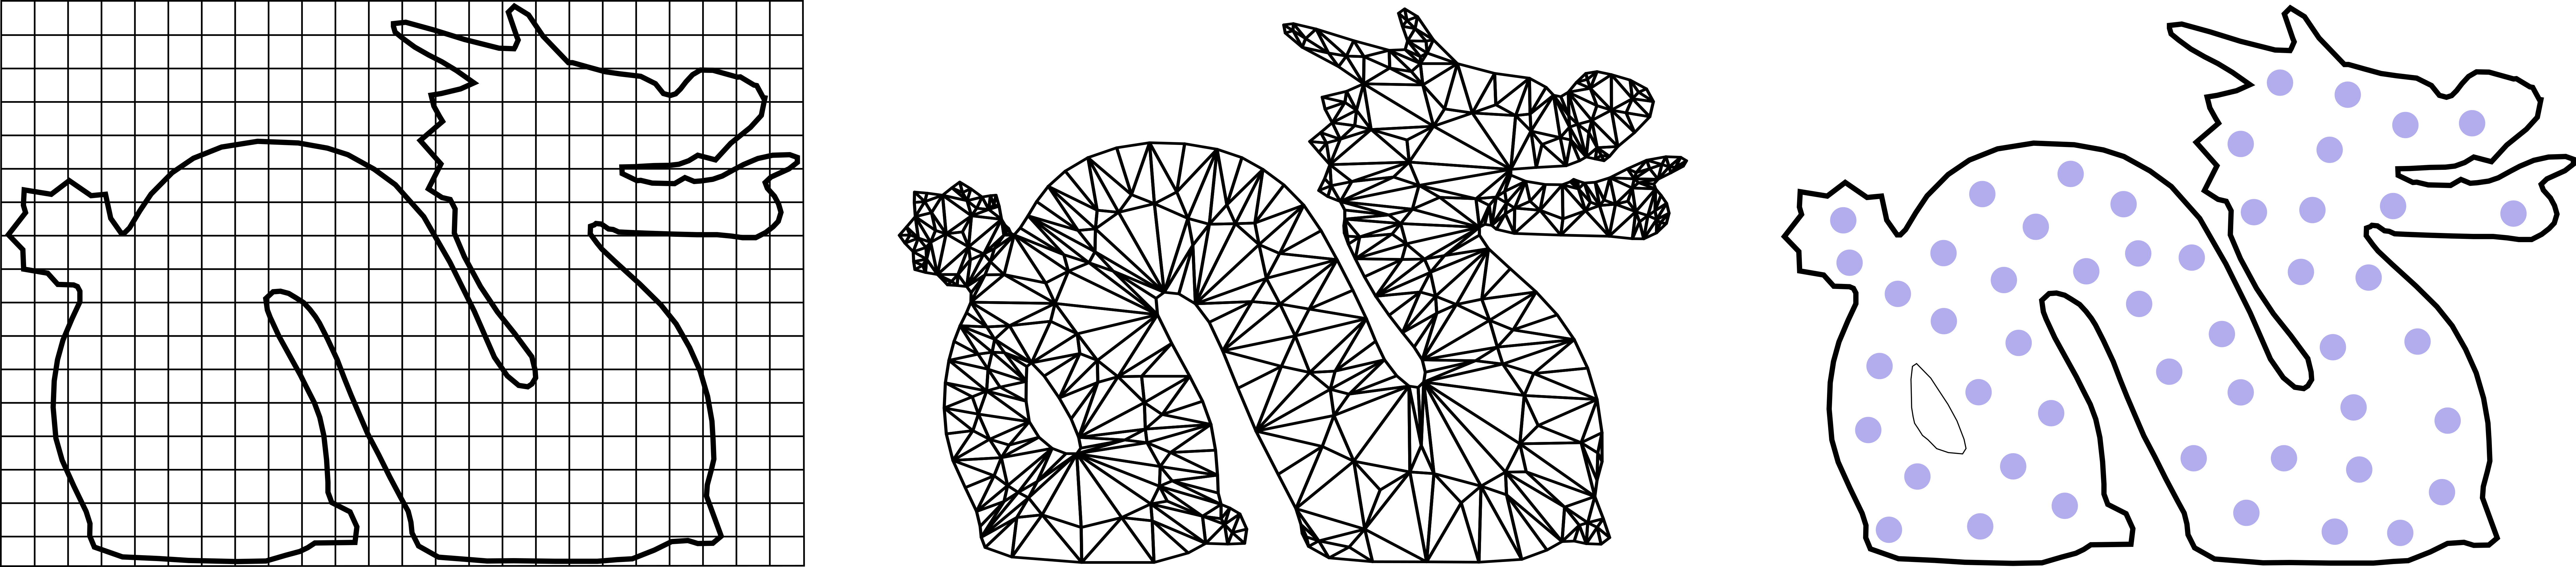
\includegraphics[width=\linewidth]{images/continuum_mechanics/discretization.png}
	\caption[STAR mechanics: Discretization]{\label{fig:discretization} On the left a grid discretization, commonly used in Eulerian simulations. In the middle an unstructured mesh discretization, commonly used in mesh-based Lagrangian simulations. On the right, a point-based discretization, commonly used in mesh-less Lagrangian simulations.}
\end{figure}
\\
In mesh-based methods, the vertices of a mesh are used to sample the degrees of freedom. For instance, Eulerian simulations usually use a cartesian grid which allows to accurately compute derivatives. 
In contrast, Lagrangian simulations are mostly based on unstructured triangular meshes which allows to handle complex boundaries.
In mesh-less methods, the samples are uniformly distributed over the domain. Depending on the simulated phenomena, the structure may be quasi-nonexistent which brings a lot of flexibility. For fluids, the neighborhood of the samples will change every time whereas for elastic solids their neighborhood will remain the same as long as the object does not undergo topological changes such as fracture or cutting.
Each of these samplings can benefit from adaptivity. We will detail the different possibilities of spatial adaptivity in Section~\ref{sec:spatial_refinement}.

\subparagraph{Interpolation}
Interpolation is used to approximate the physical quantities over the domain such as density, displacement, pressure and so on. 
In Computer Graphics, we can distinguish two major interpolation methods: polynomial interpolation and kernel interpolation.
For each of them, different weights are used, as illustrated in Figure~\ref{fig:shapefunction}. The weights are also called \emph{shape functions} and can be seen as the region of influence of a sample.
\begin{figure}[!h]
	\centering
	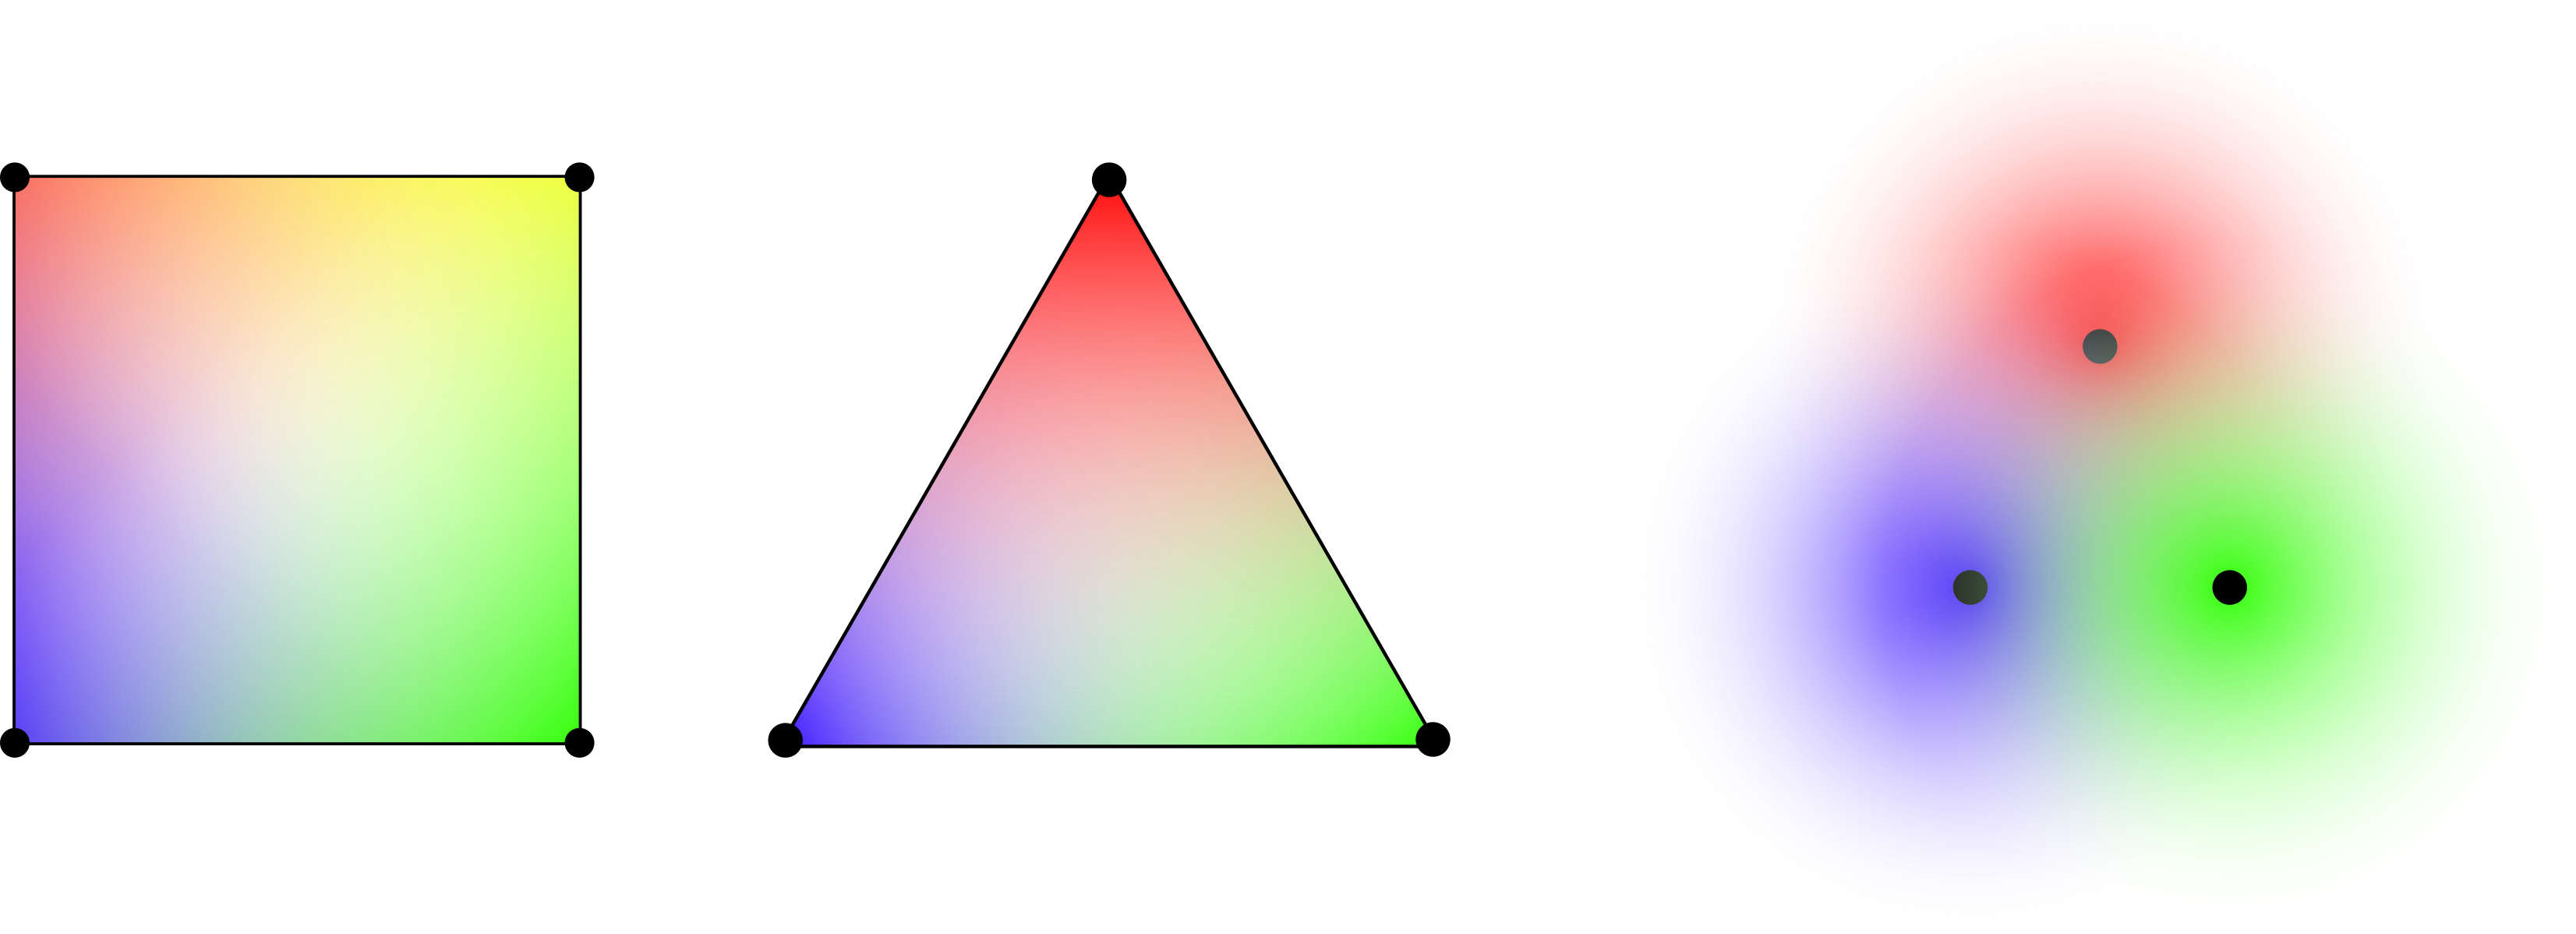
\includegraphics[width=\linewidth]{images/continuum_mechanics/shapefunction.png}
	\caption[STAR mechanics: Shape functions]{\label{fig:shapefunction} 
		Three examples of shape functions in 2D. 
		Each color represents the shape function associated to one sample point~(black circle) carrying the degrees of freedom. 
		On the left, shape functions for bilinear interpolation are illustrated. 
		In the middle, barycentric shape functions are illustrated. 
		On the right, kernel-based shape functions that are used in SPH and MLS interpolation are illustrated.}
\end{figure}
\\
The choice of the interpolation method mainly depends on how the material samples have been distributed. 
For a sampling based on cartesian grid, trilinear interpolation is often used, for instance in Eulerian simulations~\cite{Bridson2008}. 
For unstructured triangle meshes, linear interpolation with barycentric weights is the most popular choice to simulate elastic solids~\cite{Muller2008}.
For mesh-less samplings, the two most common kernel interpolation methods are Smoothed-Particle Hydrodynamics (SPH) interpolation and Moving Least Squares (MLS) interpolation.
SPH interpolation has been used to simulate a wide range of phenomena from fluid~\cite{Desbrun1999} to elastic solids~\cite{Becker2009}.
MLS has been introduced by M\"{u}ller et al. to simulate elastic and plastic deformations~\cite{Muller2004:melting}.
It was later extended to solids fracture by Pauly et al.~\cite{Pauly2005} and interactive cutting by Steinemann et al.~\cite{Steinemann2009}.
Both methods require a dense sampling of th object and can be used using a cubic kernel as shape function. We will provide more details about SPH and its use for the simulation of incompressible fluid in Section~\ref{subsubsec:starSPH} and how to save computational time by using an adaptive model in Section~\ref{sec:arps_sph}.
\\
Mesh-based and mesh-less methods can be combined to get the best of both worlds.
In this case, two interpolation methods are used, one for the mesh-based side and one for the mesh-less side.
We refer the reader to the recent \emph{SIGGRAPH} course on the material point method~\cite{Jiang2016}.
In this course, existing hybrid models are compared and the interpolation methods to transfer data from one representation  to another are described.
\\
A common drawback of the methods mentioned above is that they require a dense sampling. In Section~\ref{sec:adaptivesf}, we will detail how to interactively handle topological changes with a sparse sampling by using the Voronoi-based interpolation method used in the frame-based model.

\subparagraph{Spatial Integration}

Over the simulation, different physical quantities such as density or internal forces, need to be integrated over the domain. 
There is need for a quadrature rule. 
Many exist, most of the time the simple midpoint rule is chosen (see Figure~\ref{fig:spatialIntegration}). 
\begin{figure}[H]
	\centering
	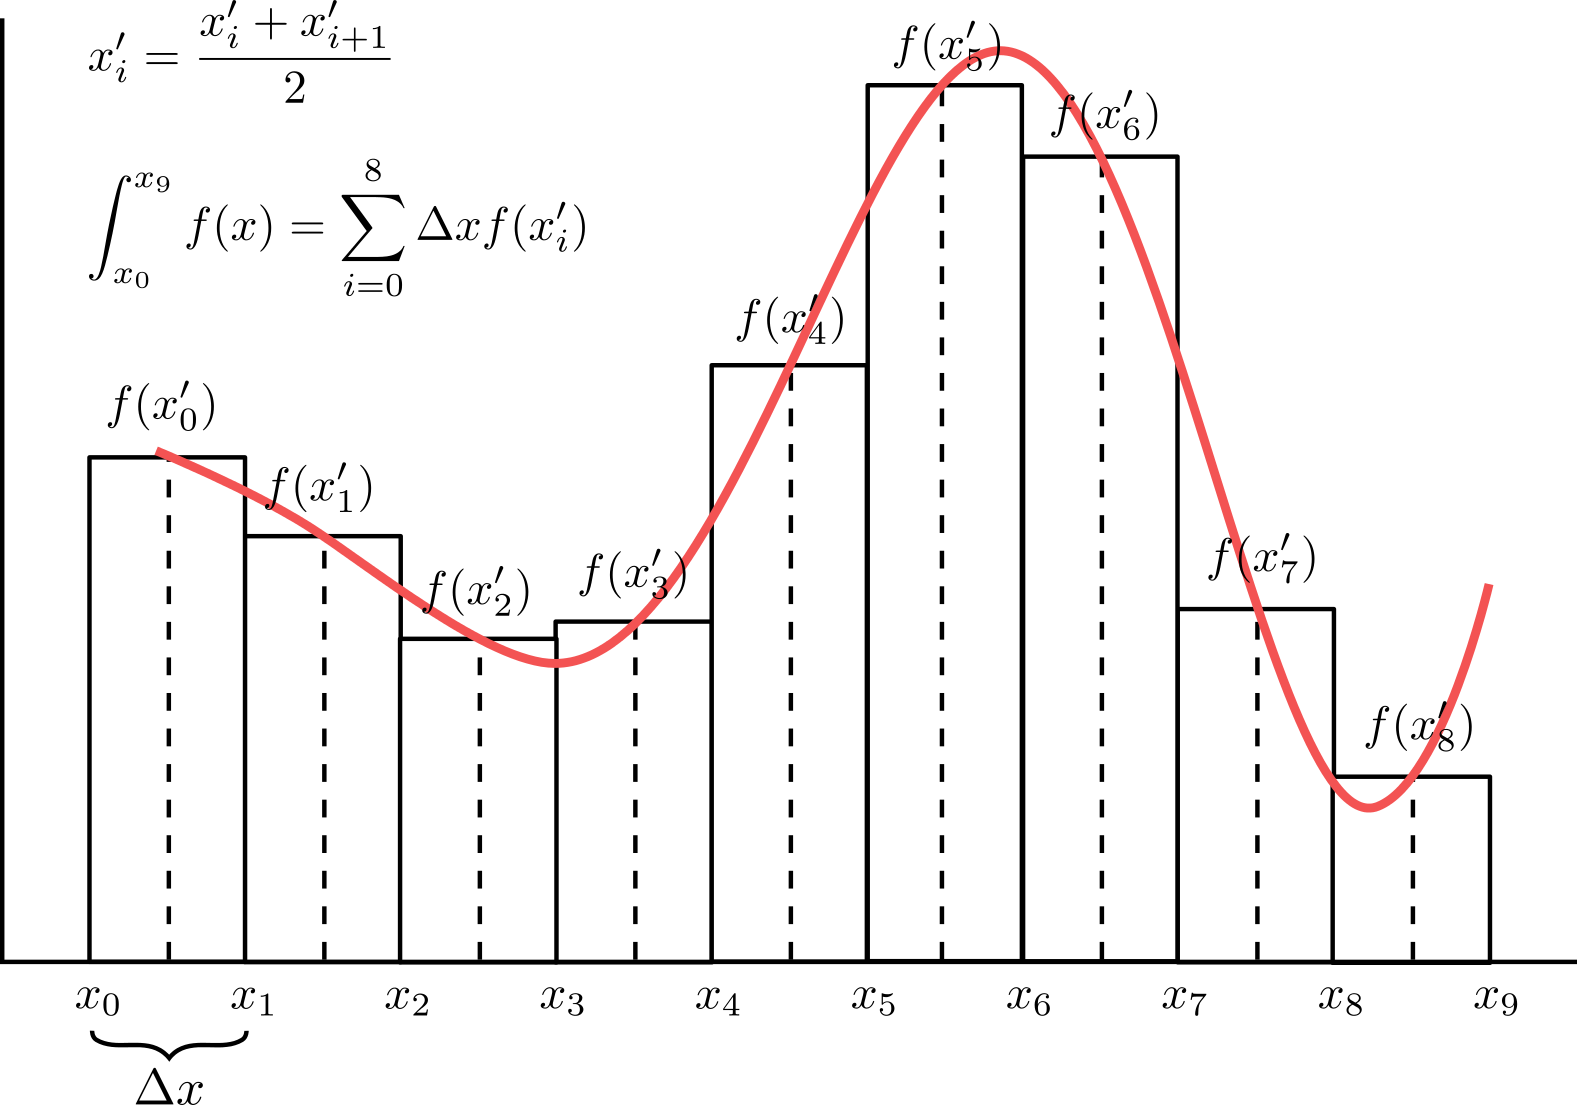
\includegraphics[width=0.8\linewidth]{images/continuum_mechanics/spatialIntegration.png}
	\caption[STAR mechanics: Spatial integration]{\label{fig:spatialIntegration} Illustration of the midpoint rule for a one dimensional function. The integration domain is partitioned into uniform regions $\left[x_{i}, x_{i+1}\right]$, an integration point $x'_{i}$ is sampled at the center of each partition and the function is evaluated at the location of the integration points.}
\end{figure}
The domain is decomposed in a set of partitions, where each partition has an associated volume $V_{i}$. 
\emph{Mid}-Points $\mathbf{x'}_{i}$ are sampled at the center of each partition.
They are called \emph{integration points}. 
Then the integral of a function $f$ over a domain $\Omega$ is approximated by:
\begin{equation}
\label{eq:midpointRule}
\int_{\Omega} f(\mathbf{x})dv \simeq \sum_{i} V_{i}f(\mathbf{x'}_{i})
\end{equation}
In mesh-based methods, it is common to consider one integration point at the center of each element and integrate over the volume of the element.
In mesh-less methods, when the sampling is dense, integration points are often co-located with the material samples and integrated over their associated volume. 
However, when the sampling is sparse, an independent sampling of integration points can be used to get a finer integration.
This is the case in the frame-based method that will be described in Section~\ref{subsubsec:framebased}.

\paragraph{Time integration}
Let us assume that we spatially discretized the Lagrangian equations of motion, Equation~\eqref{eq:lagrangianMotionEquation}, using a finite number of samples $N$ which carry positions and velocities as degrees of freedom.
For the sake of simplicity, we also assume that each sample has a fixed mass through the simulation which implies that mass conservation is ensured. Then, we can solely focus on the conservation of momentum and its integration over the time range  $\left[0, T\right]$ of the simulation. 
\\ 
As for spatial integration, the temporal domain is discretized. Ideally, this discretization would adapt to the time scale of the simulation. For instance, fast motion would require a fine discretization while a coarse discretization would be sufficient for slow motion. We will detail the different techniques for an adaptive discretization of time in Section~\ref{sec t adaptivity}.
In the following, we simply assume a uniform discretization of $\left[0,T\right]$ defined by a time step $\Delta t$. The integration between two consecutive time steps $t_{n}$ and $t_{n+1}$ can be written as
\begin{equation}
\label{eq:timeIntegration1}
\displaystyle
\int_{t_{n}}^{t_{n+1}}
M \frac{d\mathbf{v}}{dt} dt
=
\int_{t_{n}}^{t_{n+1}}\mathbf{f} dt
\end{equation}
where
\begin{itemize}
	\item $\mathbf{v} \in \mathbb{R}^{3N}$ concatenates the velocity of each sample.
	\item $\mathbf{f} \in \mathbb{R}^{3N}$ concatenates the forces applied on each sample.
	\item $M \in \mathbb{R}^{3N \times 3N}$ concatenates the mass of each sample.
\end{itemize}
Many integration schemes can be used. Most of them can be explained using the Taylor expansion of a function $f$,
\begin{equation}
\label{eq:taylorExpansion}
\displaystyle
f(x) = \sum_{\alpha=0}^{k}\frac{\left(x-a\right)^{\alpha}}{\alpha!}f^{(\alpha)}(a) + \int_{a}^{x}\frac{\left(x-t\right)^{k}}{k!}f^{(k+1)}(t)dt
\end{equation}
By applying Equation~\eqref{eq:taylorExpansion} on $\mathbf{v}$ with $k=0$, we have
\begin{equation}
\mathbf{v}(t_{n+1}) = \mathbf{v}(t_{n}) + \int_{t_{n}}^{t_{n+1}} \frac{d\mathbf{v}}{dt}dt
\end{equation}
which allows to rewrite Equation~\eqref{eq:timeIntegration1} as
\begin{equation}
\label{eq:timeIntegration2}
\mathbf{v}(t_{n+1}) = \mathbf{v}(t_{n}) + \int_{t_{n}}^{t_{n+1}} M^{-1}\mathbf{f}dt
\end{equation}
This expression can be further expanded in order to get more accurate results. In Computer Graphics, this is the most used expansion. Finally, the integral term in Equation~\eqref{eq:timeIntegration2} is generally computed with the rectangle quadrature rule which we illustrate in Figure~\ref{fig:rectangleRules}.
\begin{figure}[!ht]
	\centering
	\begin{subfigure}[b]{0.46\linewidth}
		\centering
		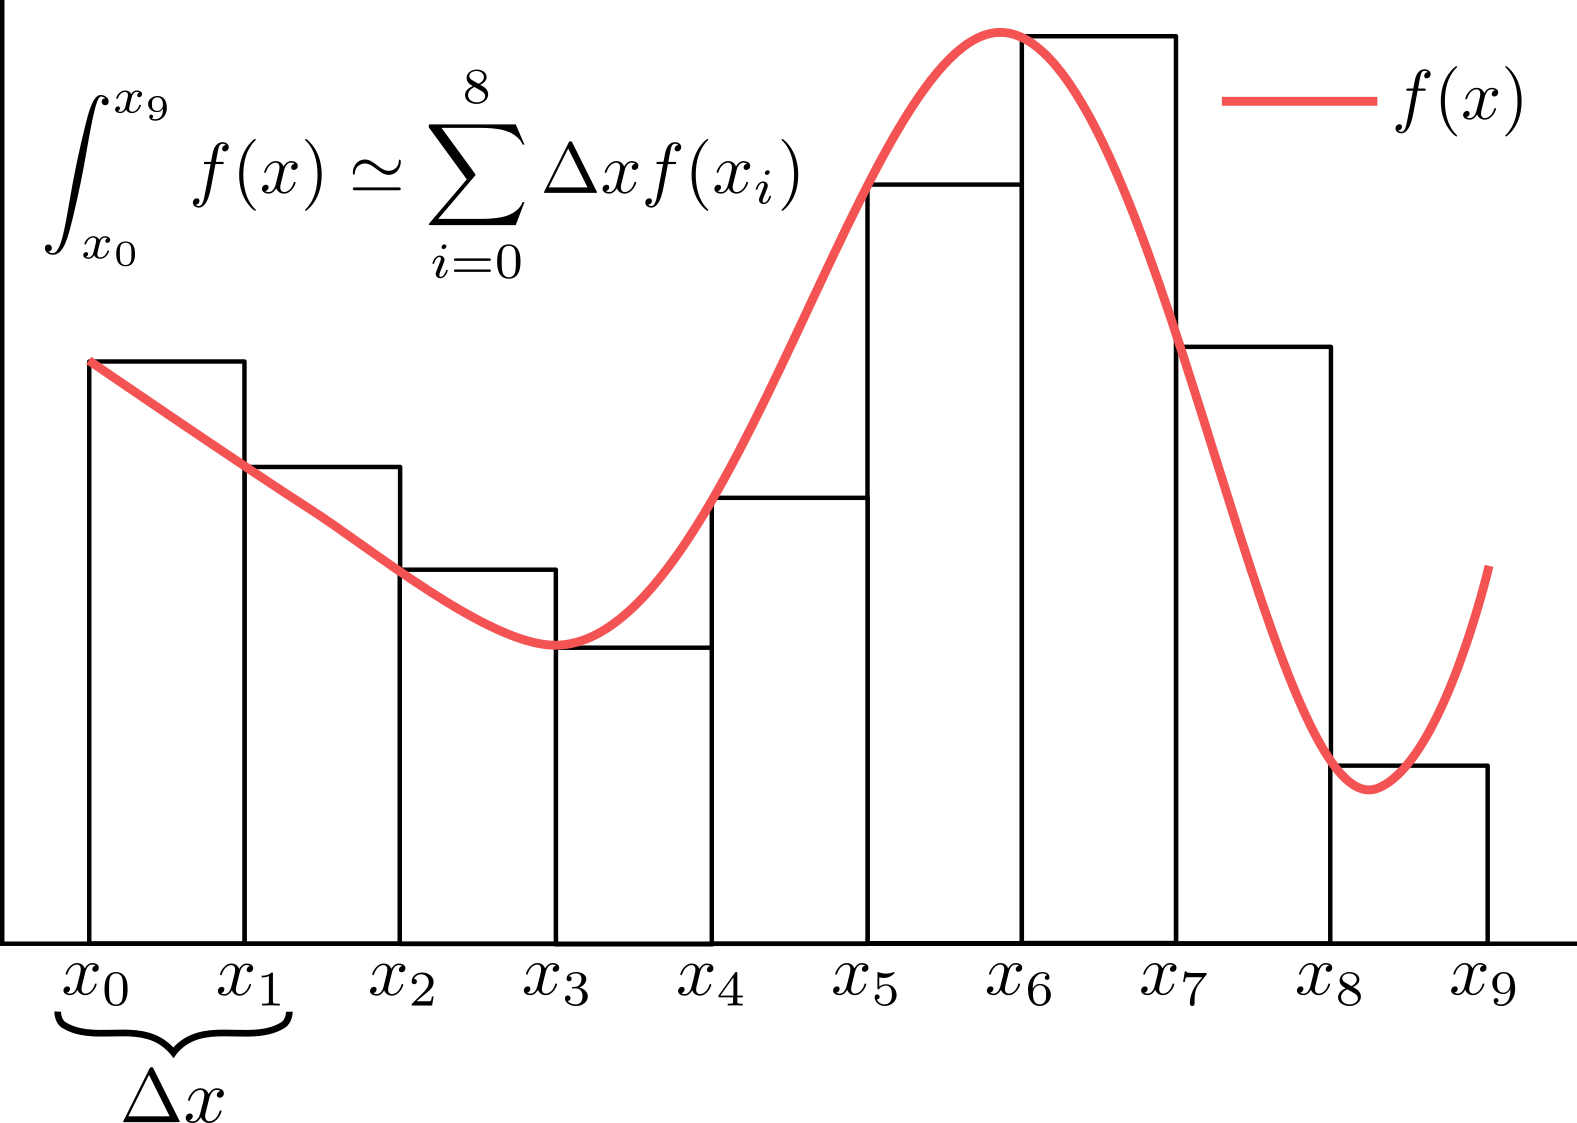
\includegraphics[width=\linewidth]{images/continuum_mechanics/rectangleRule_left.png}
		\caption{\label{fig:leftRectangleRule}}
	\end{subfigure}
	\hspace{0.2cm}
	\begin{subfigure}[b]{0.46\linewidth}
		\centering
		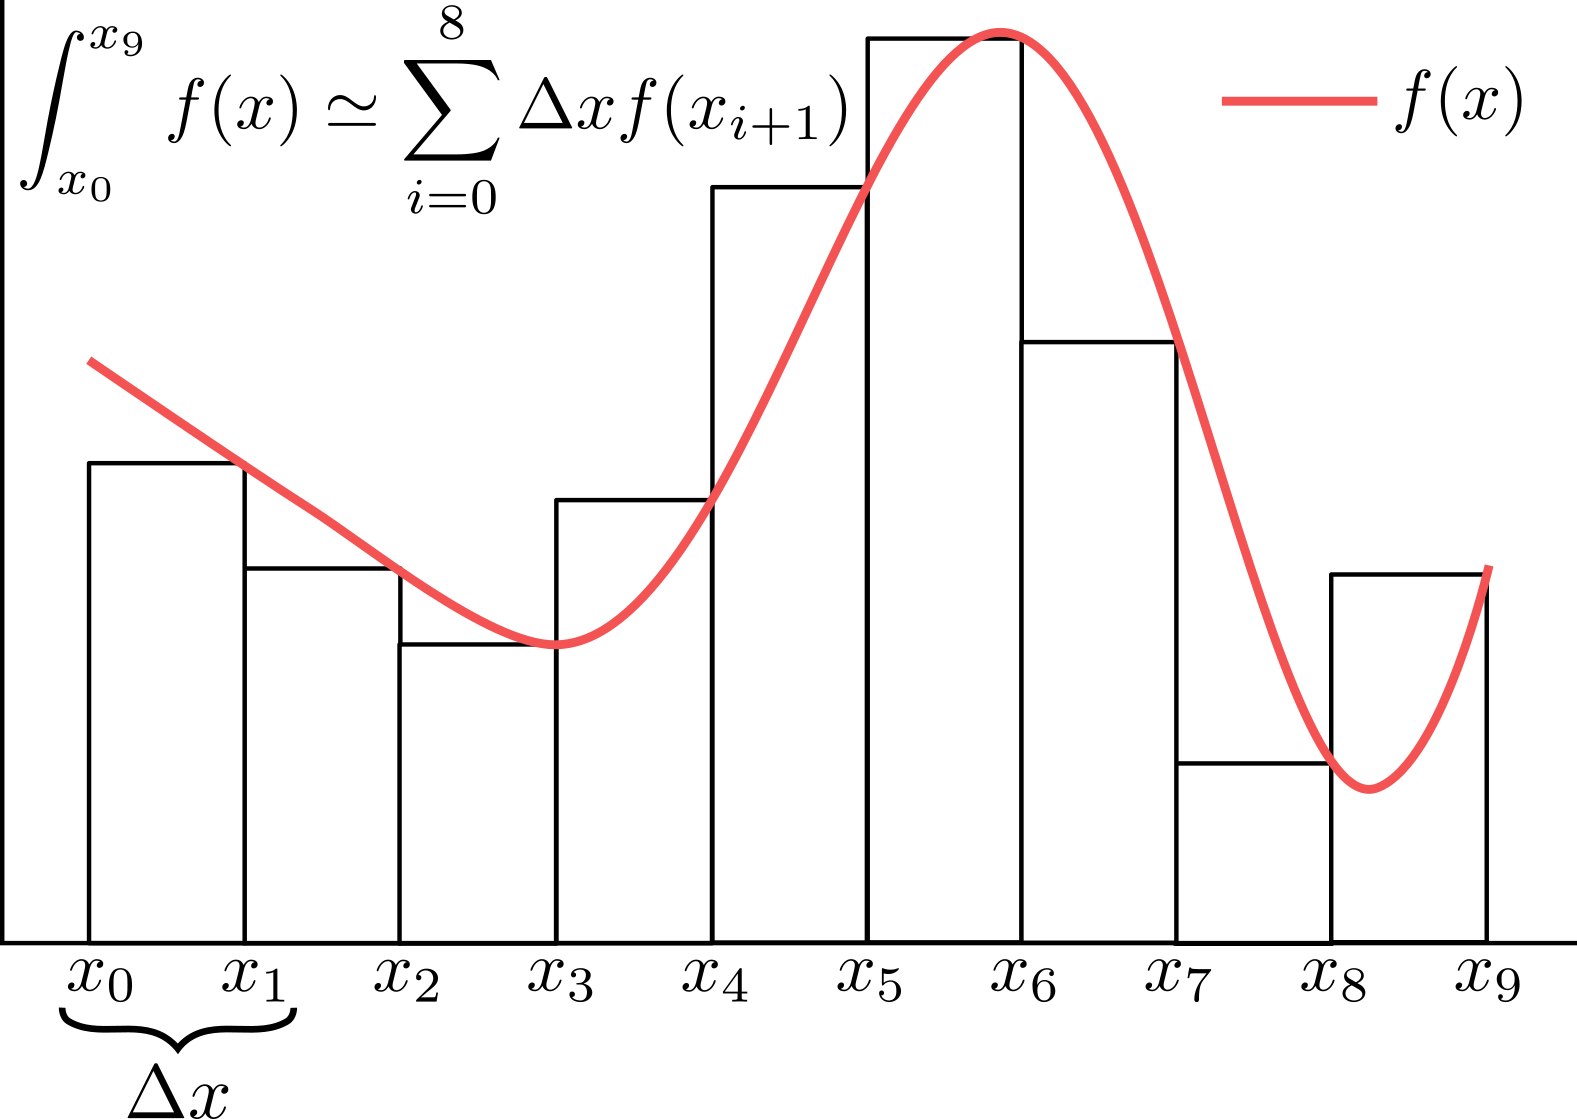
\includegraphics[width=\linewidth]{images/continuum_mechanics/rectangleRule_right.png}
		\caption{\label{fig:rightRectangleRule}}
	\end{subfigure}
	\caption[STAR mechanics: Rectangle integration rules]{\label{fig:rectangleRules}
		Illustrations of the rectangle integration rules. A function $f$ can be integrated over a regularly sampled domain using either the left rectangle rule~(a) or the right rectangle rule~(b).}
\end{figure}
\\
For a left rectangle method, we get an explicit integration of the velocity
\begin{equation}
\label{eq:explicitIntegration}
\mathbf{v}(t_{n+1}) = \mathbf{v}(t_{n}) + \Delta t M^{-1}\mathbf{f}(t_{n})
\end{equation}
For a right rectangle method, we get an implicit integration of the velocity
\begin{equation}
\label{eq:implicitIntegration}
\mathbf{v}(t_{n+1}) = \mathbf{v}(t_{n}) + \Delta t M^{-1}\mathbf{f}(t_{n+1})
\end{equation}
We can apply the same rule for the integration of the positions.
Depending on which quantity is integrated first and which integration rule is used, we can distinguish three main schemes used in computer graphics: forward Euler, symplectic Euler and backward Euler.
\begin{figure}[!ht]
	\centering
	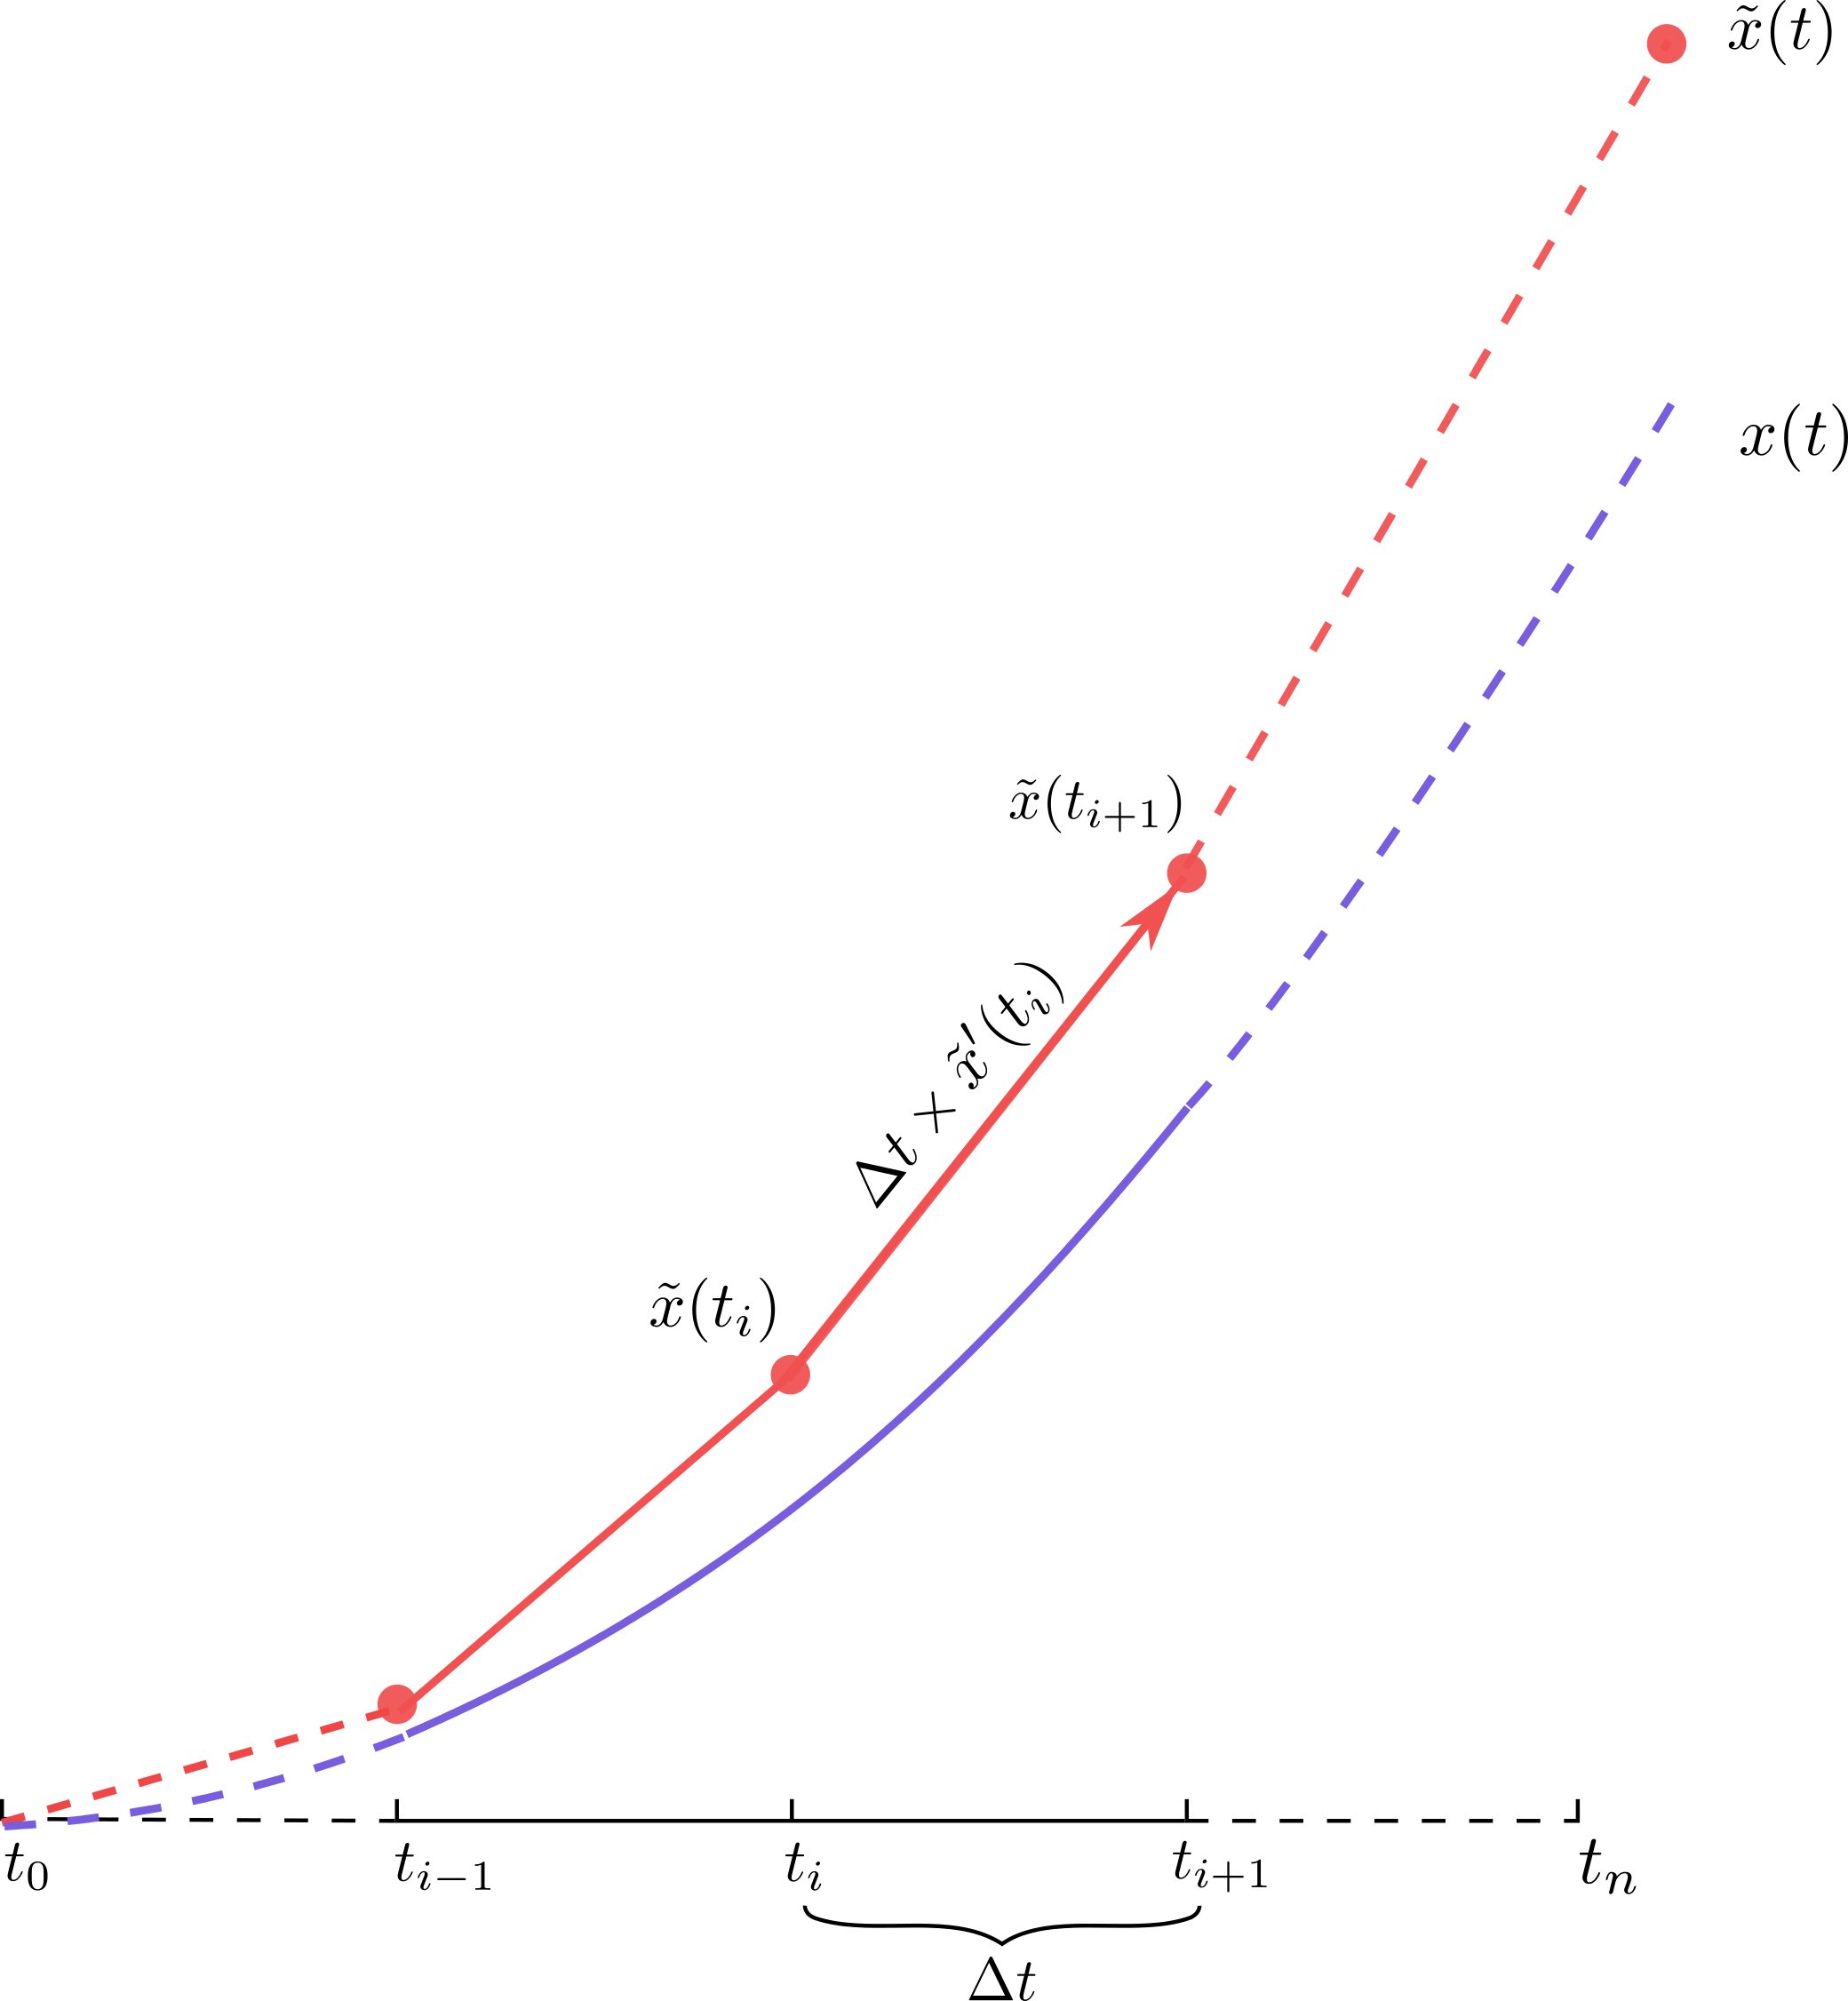
\includegraphics[scale=0.6]{images/continuum_mechanics/timeIntegration.png}
	\caption[STAR mechanics: Temporal integration]{\label{fig:timeIntegration} 
		Illustration of a 1D forward Euler time integration. 
		$x(t)$ describes the solution and $x'(t)$ describes the numerical approximation.}
\end{figure}
Forward Euler is the explicit integration of both position and velocity.
Figure~\ref{fig:timeIntegration} illustrates the integration of position in 1D,
\begin{equation}
\label{eq:explicitEuler}
\begin{array}{l}
\displaystyle \mathbf{x}(t_{n+1}) = \mathbf{x}(t_{n}) + \Delta t \mathbf{v}(t_{n}) \\ \\
\displaystyle \mathbf{v}(t_{n+1}) = \mathbf{v}(t_{n}) + \Delta t M^{-1}\mathbf{f}(t_{n})
\end{array}
\end{equation}
Symplectic Euler is the explicit integration of velocity and implicit integration of position,
\begin{equation}
\label{eq:symplecticEuler}
\begin{array}{l}
\displaystyle \mathbf{v}(t_{n+1}) = \mathbf{v}(t_{n}) + \Delta t M^{-1} \mathbf{f}(t_{n}) \\ \\
\displaystyle \mathbf{x}(t_{n+1}) = \mathbf{x}(t_{n}) + \Delta t \mathbf{v}(t_{n+1})
\end{array}
\end{equation}
Backward Euler is the implicit integration of both position and velocity,
\begin{equation}
\label{eq:backwardEuler}
\begin{array}{ll}
\displaystyle \mathbf{v}(t_{n+1}) = \mathbf{v}(t_{n}) + M^{-1}\Delta t \mathbf{f}(t_{n+1}) \\ \\
\displaystyle \mathbf{x}(t_{n+1}) = \mathbf{x}(t_{n}) + \Delta t \mathbf{v}(t_{n+1})
\end{array}
\end{equation}
On one hand, forward and symplectic Euler are easy to implement and cheap to compute but stability is guaranteed for a restricted range of time steps. 
On the other hand, backward Euler is more expensive as it requires the solution of an equation but this is greatly compensated by the larger time steps which can be used while ensuring stability.
However, this speed-up comes at the price of numerical damping which might be undesired.
A nice way to solve the non-linear equation of backward Euler is to expand the force expression and linearize in order to fall back to solving a linear system. There, efficient iterative methods such as the conjugate gradient can be used.
In Section~\ref{sec:arps_implicit}, we describe the linear system resulting from the use of backward Euler and detail how to combine it with the adaptive method that we present in Chapter~\ref{chap:arps}.

\subsection{Fluid mechanics}
\label{subsec:fluidMechanics}
In this section, we describe a constitutive law for incompressible fluids such as water and we detail how to solve the equations of motion by using the Smoothed-Particle Hydrodynamics~(SPH) model that we will use in Section~\ref{sec:arps_sph}.
\subsubsection{Constitutive Law}
Fluids, for instance smoke, mainly react to pressure and viscosity.
The stress tensor that we introduced in Section~\ref{subsubsec:starMechanics_momentumConservation} is used to relate the deformation of the fluid to this two properties in the following constitutive law
\begin{equation}
\label{eq:fluidConstitutiveLaw}
\sigma = -pI + \eta \left( \nabla \mathbf{v} + \nabla \mathbf{v}^{T} \right)
\end{equation}
where
\begin{itemize}
	\item $p$ is the pressure applied on the fluid.
	\item $\eta$ is the viscosity of the fluid.
\end{itemize}
By injecting this equation into Equation~\eqref{eq:internalForces}, we get the internal forces of the fluid:
\begin{equation}
\label{eq:internalForces_liquids}
\mathbf{f}_{int} = \nabla \cdot \sigma = \nabla \cdot \left( -pI + \eta \left( \nabla \mathbf{v} + \nabla \mathbf{v}^{T} \right) \right) = -\nabla p + \Delta \mathbf{v}
\end{equation}
If we want to describe an incompressible fluid such as water, we need to specify that the mass should not vary over time which means
\begin{equation}
\label{eq:incompressibility}
\frac{d\rho}{dt} = 0
\end{equation}
By using Equation~\eqref{eq:internalForces_liquids}~and~\eqref{eq:incompressibility} in the equations of motion described in Equation~\eqref{eq:lagrangianMotionEquation}, we now describe an incompressible fluid. These new equations of motion are called the Navier-Stokes equations for an incompressible fluid
\begin{equation}
\label{eq:navierStokes}
\left\lbrace
\begin{array}{ll}
\displaystyle \int_{\mathcal{V}} \left( \rho \frac{d}{dt} \mathbf{v} + \nabla p - \eta \Delta \mathbf{v} - \rho \mathbf{g} \right)dv = \mathbf{0}\\ \\
\displaystyle \int_{\mathcal{V}} \nabla. \mathbf{v} dv = 0
\end{array}
\right.
\end{equation}
\subsubsection{Smoothed-Particle Hydrodynamics model}
\label{subsubsec:starSPH}
Smoothed-Particle Hydrodynamics (SPH) is an interpolation method that can be used to approximate Navier-Stokes equations in a Lagrangian way. 
SPH was initially proposed by Monaghan~\cite{Monaghan1992} and introduced in graphics by Desbrun et al.~\cite{Desbrun1999}.
The fluid is discretized into particles which represent small volumes of the whole fluid and each quantity carried by the particle is interpolated using SPH.
In Chapter~\ref{chap:arps}, we will describe how to easily combine SPH with an adaptive model in order to save computational time.
\paragraph{SPH interpolation}
The interpolation of a function $f$ and its derivatives of order $\alpha$ at a position $\mathbf{x}$ using SPH are defined as
\begin{equation}
\label{eq:sphInterpolation}
\left\lbrace
\begin{array}{l}
\displaystyle f(\mathbf{x}) = \int_{V} f(\mathbf{x'})W(\mathbf{x}-\mathbf{x'}, h)d\mathbf{x'} \\ \\
\displaystyle D^{\alpha} f(\mathbf{x}) = \int_{\mathcal{V}} f(\mathbf{x'}) D^{\alpha} W(\mathbf{x}-\mathbf{x'}, h)d\mathbf{x'}
\end{array}
\right.
\end{equation}
where 
\begin{itemize}
	\item $W$ is a function called \emph{kernel}.
	\item $h$ is the smoothing radius, also called length scale, which represents the support of $W$.
\end{itemize} 
Let assume that the fluid is discretized using $N$ particles.
These particles play two roles: First they carry the degrees of freedom and the fluid properties; Second their position are used as integration points. By applying the midpoint rule from Equation~\eqref{eq:midpointRule}, we get a discretized version of Equation~\eqref{eq:sphInterpolation}:
\begin{equation}
\label{eq:sphFunction}
\left\lbrace
\begin{array}{l}
\displaystyle f(\mathbf{x}) = \sum_{i=0}^{N} f(\mathbf{x}_{i})V_{i} W(\mathbf{x}-\mathbf{x}_{i},h) \\ \\
\displaystyle D^{\alpha} f(\mathbf{x})= \sum_{i=0}^{N} f(\mathbf{x}_{i})V_{i} D^{\alpha} W(\mathbf{x}-\mathbf{x}_{i},h)
\end{array}
\right.
\end{equation}
where 
\begin{itemize}
	\item $V_{i} = m_{i}/\rho_{i}$ is the volume of particle $i$.
	\item $m_{i}$ is the mass of particle $i$.
	\item $\rho_{i}$ is the density of particle $i$.
\end{itemize}
\paragraph{How to choose the kernel}
The choice of the kernel varies depending on the function to interpolate. In practice, the cubic kernel from Monaghan~\cite{Monaghan1992}~(Figure~\ref{fig:cubicKernel}) that we use in Chapter~\ref{chap:arps} works well.
\begin{figure}[!h]
	\centering
	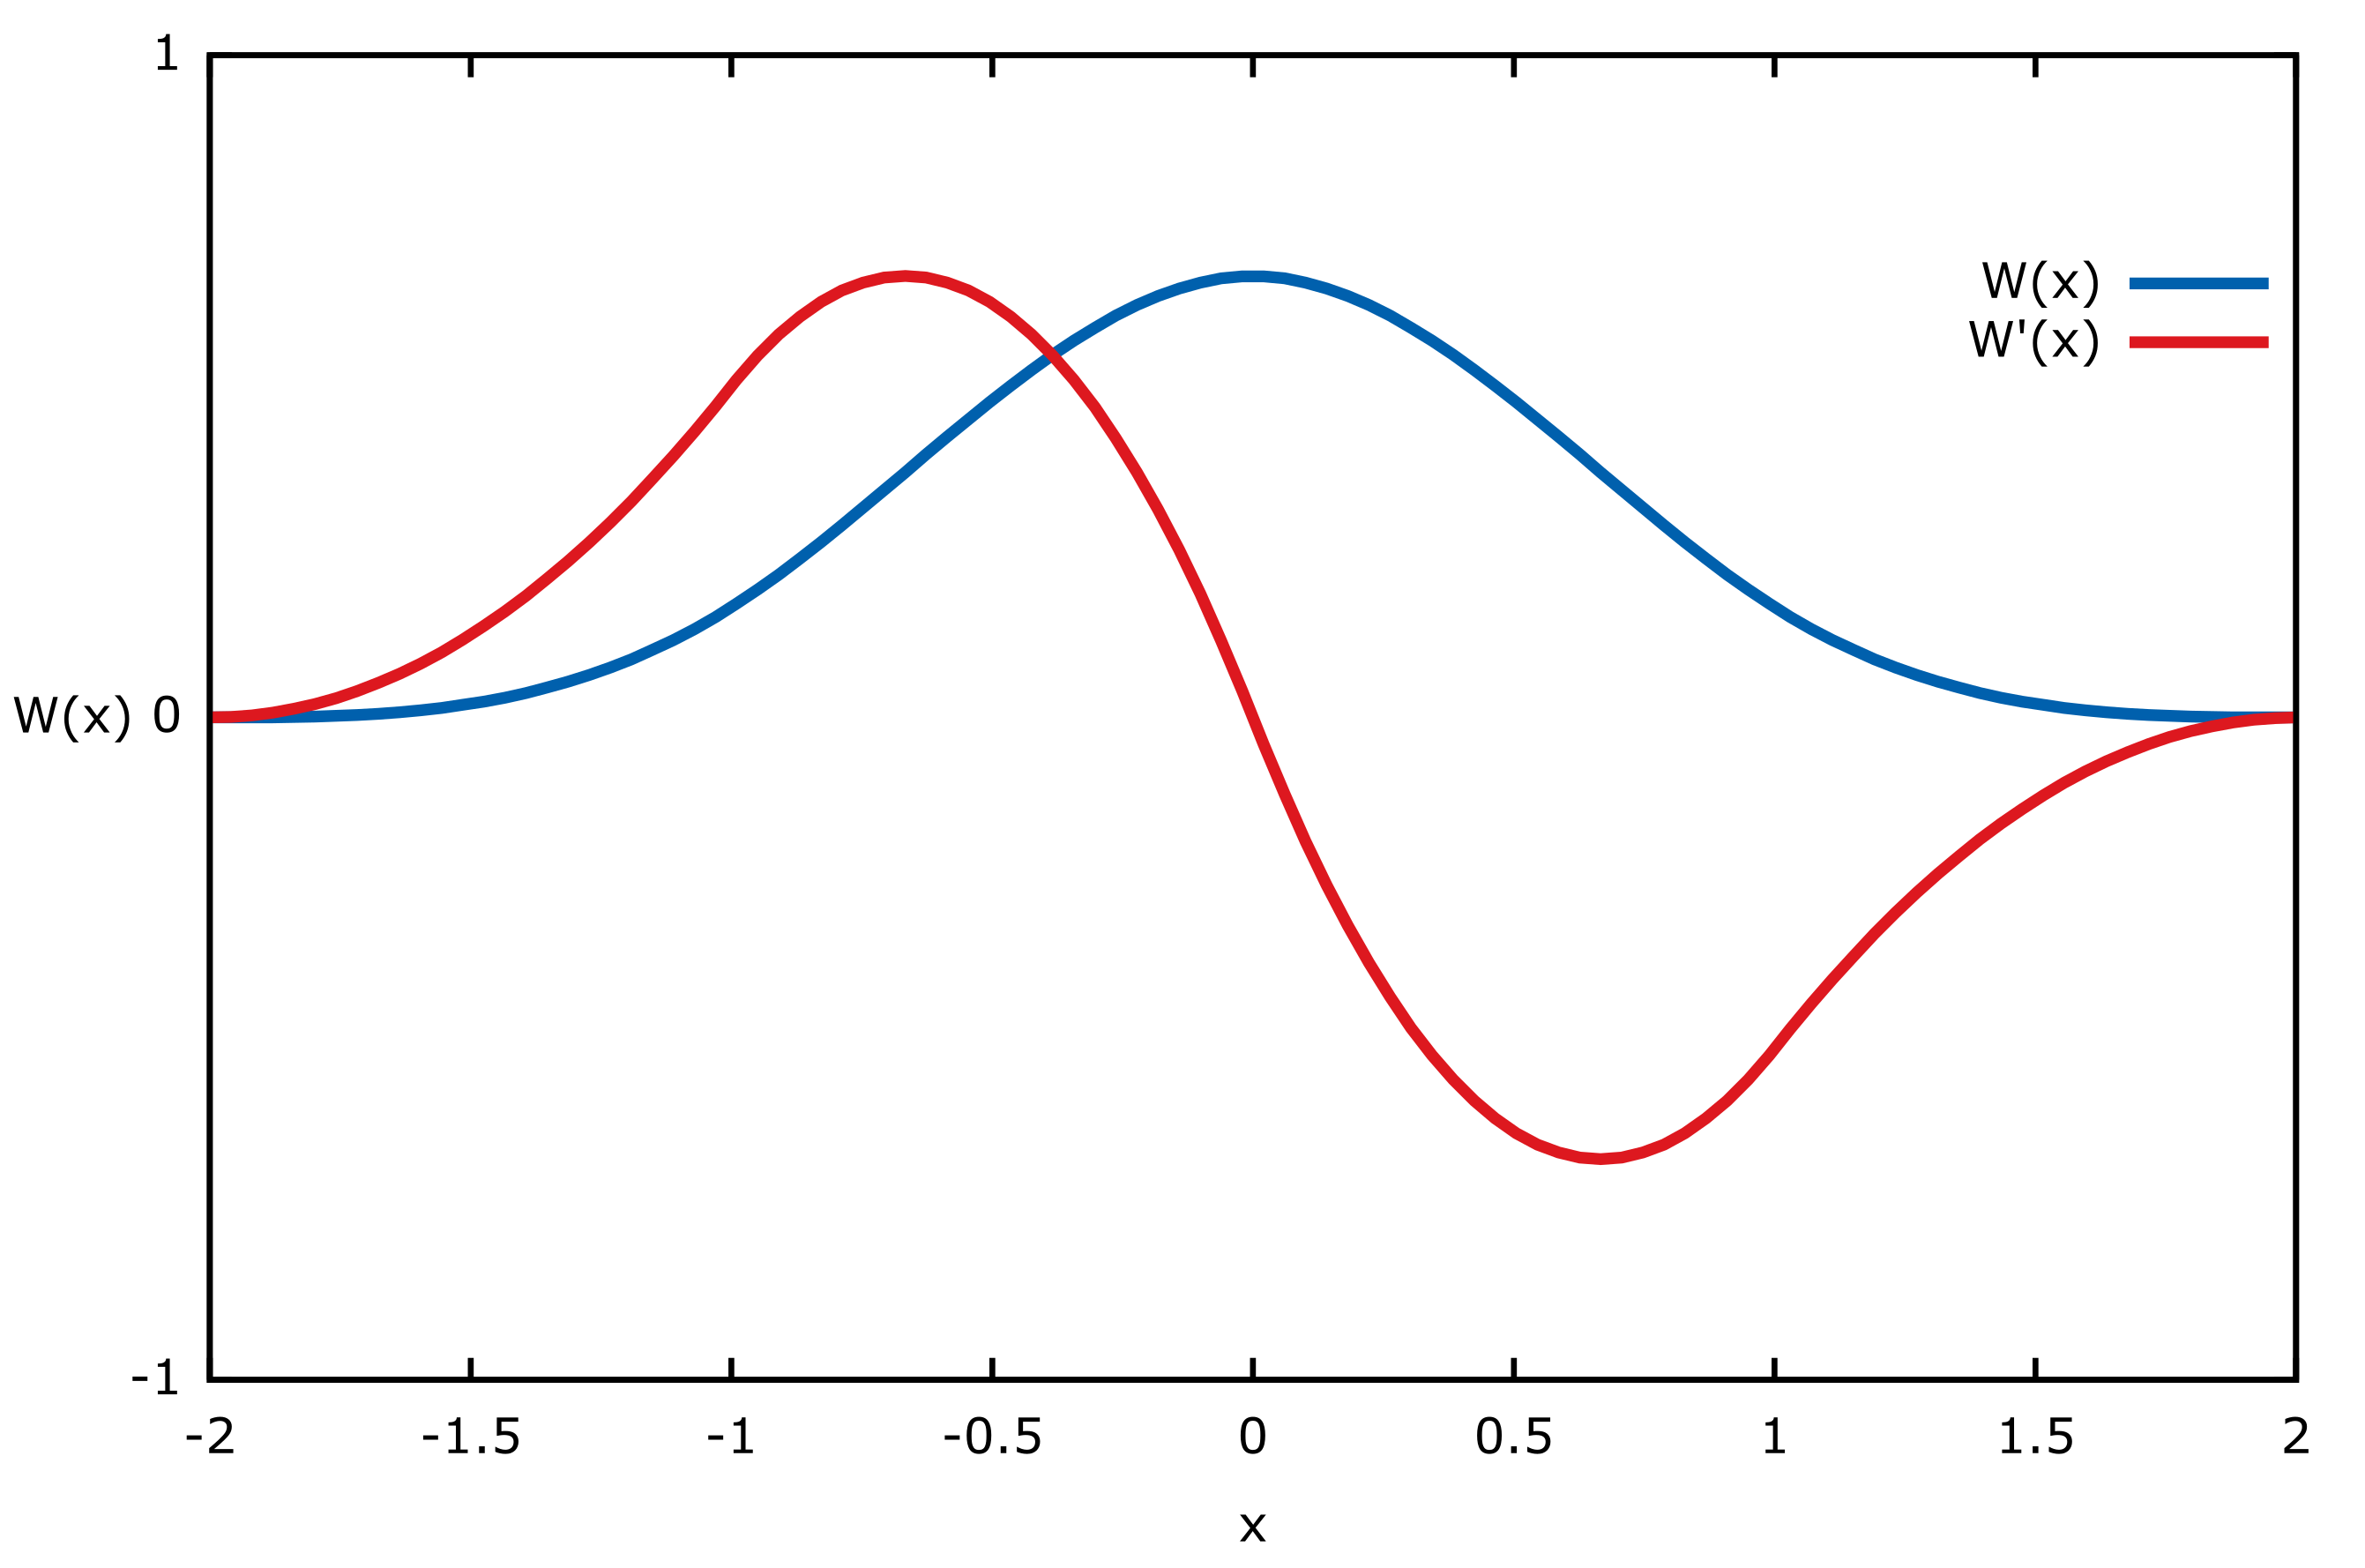
\includegraphics[width=\linewidth]{images/continuum_mechanics/cubicKernel.png}
	\caption[STAR mechanics: Cubic kernel]{\label{fig:cubicKernel}
		Illustration of the 1D cubic kernel used by Monaghan et al.~\cite{Monaghan1992} and its derivative for $h=1$. Note that the support of $W$ is $2h$.}
\end{figure}
This kernel meets properties which are generally required from $W$
\begin{itemize}
\item $W$ is normalized. Thus, constants are interpolated exactly.
\item $W$ has a compact support.
\begin{equation}
\parallel \mathbf{x} \parallel \geq h \implies W(\mathbf{x},h) = 0 
\end{equation}
\begin{equation}
\int_{\mathcal{V}} W(\mathbf{x},h) dx = 1
\end{equation}
\item $W$ tends to the delta function when the length scale $h$ tends to $0$.
\begin{equation}
\lim_{h \rightarrow 0} W(x,h) = \delta(x)
\end{equation}
\item $W$ should be symmetric to enforce invariance under rotation
\begin{equation}
W(-x,h) = W(x,h)
\end{equation}
\item Depending on the function to interpolate the kernel should be positive to prevent unphysical interpolated value.
\begin{equation}
W \geq 0
\end{equation}
\end{itemize}
Here we can notice a first limitation of SPH: For a constant function $f$, the approximation of its first derivatives using Equation~\eqref{eq:sphFunction} will not necessarily vanish depending on $W$. A common practice to fix that is to consider the derivative of the product of $f$ with an arbitrary differentiable function that we note $\Phi$
\begin{equation}
\label{eq:hackSPH}
\nabla f = \frac{1}{\Phi}\left(\nabla (f \Phi) - f \nabla \Phi \right)
\end{equation}
In this case, we can approximate $\nabla(f\Phi)$ and $\nabla \Phi$ using Equation~\eqref{eq:sphFunction}. If $f$ is constant, we will get $\nabla f = 0$. In practice the density $\rho$ is often used for $\Phi$. In the following paragraph, we will see another usage of this technique.
\paragraph{Application to Navier-Stokes equations}
First of all, let us discretize Navier-Stokes equation on the sampling of the particles using the midpoint rule:
\begin{equation}
\label{eq:particleNavierStokes}
\left\lbrace
\begin{array}{ll}
\displaystyle \sum_{i=0}^{N} \left( \rho_{i} \frac{d}{dt} \mathbf{v}_{i} + \nabla p_{i} - \eta \Delta \mathbf{v}_{i} - \rho_{i} \mathbf{g} \right) V_{i} = \mathbf{0}\\ \\
\displaystyle \sum_{i=0}^{N} \nabla. \mathbf{v}_{i} V_{i} = 0
\end{array}
\right.
\end{equation}
We can omit the mass conservation as we did before, by assuming that the particles have a fixed mass through the simulation. Recently, Bender and Koschier~\cite{Bender2015} demonstrated that this simplification prevents from using larger time steps. But for the sake of simplicity, we will keep this approximation in the remainder of this manuscript. Now, we can discretize each term of the equations for a particle $i$ using the SPH technique from Equation~\eqref{eq:sphFunction}.
\subparagraph{Density}
\begin{equation}
\label{eq:densitySPH}
\rho_{i} = \sum_{j=0}^{N} m_{j}W(\mathbf{x_{i}}-\mathbf{x_{j}},h)
\end{equation}
\subparagraph{Pressure}
\begin{equation}
\label{eq:pressureSPH}
p_{i} = k\left(\rho_{i}-\rho_{0}\right)
\end{equation}
where 
\begin{itemize}
\item $\rho_{0}$ is the rest density of the fluid ($1000\kilo\gram\per\meter\cubed$).
\item $k$ is a stiffness parameter.
\end{itemize}
Equation~\eqref{eq:pressureSPH} is a simple and cheap computation of the pressure. This equation of state acts like a spring in order to enforce the incompressibility of the fluid.
However, a high stiffness is generally needed to get close to incompressibility. Therefore, very small time steps are required to ensure stability. Recently, new techniques were proposed to ensure incompressibility while using larger time steps. We do not detail these methods in this manuscript but refer the reader to the work of Ihmsen et al.~\cite{Ihmsen2014:IISPH} and Bender and Koschier~\cite{Bender2015}.
\subparagraph{Pressure gradient}
\begin{equation}
\left(\nabla p\right)_{i} = \sum_{j=0}^{N} \frac{m_{j}}{\rho_{j}} p_{j} \nabla W(\mathbf{x_{i}}-\mathbf{x_{j}},h)
\end{equation}
Here we can notice that the resulting pressure force between two particles $i$ and $j$ is not symmetric and therefore does not conserve linear and angular momentum:
\begin{equation}
\label{eq:nonSymmetricPressureForce}
\mathbf{f}^{pressure}_{ij} = -\frac{m_{i}m_{j}}{\rho_{i}\rho_{j}}p_{j}\nabla W(\mathbf{x_{i}}-\mathbf{x_{j}},h)
\end{equation}
To remedy this problem, we can use Equation~\eqref{eq:hackSPH} with $\displaystyle \Phi = \frac{1}{\rho_{i}}$
\begin{equation}
\left(\nabla p\right)_{i} = \rho_{i} \left( \nabla \left(\frac{p_{i}}{\rho_{i}}\right) + p_{i}\frac{\nabla \rho_{i}}{\rho_{i}^{2}}\right)
\end{equation}
and re-use SPH interpolation to get a new approximation of the pressure gradient
\begin{equation}
\label{eq:pressureGradientSPH}
\left(\nabla p\right)_{i} = 
\rho_{i}
\sum_{j=0}^{N} m_{j} \left( \frac{p_{i}}{\rho_{i}^{2}} + \frac{p_{j}}{\rho_{j}^{2}} \right) \nabla W(\mathbf{x_{i}}-\mathbf{x_{j}},h)
\end{equation}
which results into symmetric pressure forces between two particles $i$ and $j$:
\begin{equation}
\label{eq:symmetricPressureForce}
\mathbf{f}^{pressure}_{ij} = 
-m_{i}m_{j}
\left( 
\frac{p_{i}}{\rho_{i}^{2}} + \frac{p_{j}}{\rho_{j}^{2}} 
\right) 
\nabla W(\mathbf{x_{i}}-\mathbf{x_{j}},h)
\end{equation}
\subparagraph{Velocity Laplacian}
\begin{equation}
\left(\Delta \mathbf{v}\right)_{i} = \sum_{j=0}^{N} \frac{m_{j}}{\rho_{j}} \mathbf{v}_{j} \Delta W(\mathbf{x_{i}}-\mathbf{x_{j}},h)
\end{equation}
Same as for the pressure gradient, this would result in a non-symmetric inter-particle viscosity force:
\begin{equation}
\label{eq:nonSymmetricViscosityForce}
\mathbf{f}^{viscosity}_{ij} = \eta\frac{m_{i}m_{j}}{\rho_{i}\rho_{j}}\mathbf{v}_{j}\Delta W(\mathbf{x_{i}}-\mathbf{x_{j}},h)
\end{equation}
If we assume that the density is constant, which is the case in theory, we could obtain symmetric forces by using Equation~\eqref{eq:hackSPH} with $\Phi=\rho_{i}$. However, in practice, the density is not constant and the evaluation of the Laplacian of the kernel is sensitive to particles sampling, which makes this solution inadequate.
Actually, it is quite hard to correctly handle viscosity using SPH and this is still an area of research, especially for liquids exhibiting complex viscous behaviors such as coiling or buckling.
We refer the reader to the recent work of Peer et al.~\cite{Peer2015} and Takahashi et al.~\cite{Takahashi2015} about this topic.
For fluid with a low viscosity, Monaghan~\cite{Monaghan2005} proposed a gradient-based formulation of the Laplacian which results in symmetric forces,
\begin{equation}
\label{eq:velocityLaplacianSPH}
\left(\Delta \mathbf{v}\right)_{i} = 
\frac{1}{\rho_{i}}
\sum_{j=0}^{N} m_{j} \Pi_{ij} \nabla W(\mathbf{x_{i}}-\mathbf{x_{j}},h)
\end{equation}
where 
\begin{equation}
    \Pi_{ij} = -\frac{2hc_{s}}{\rho_{i}+\rho_{j}}\frac{\mathbf{v}_{ij}^{T}\mathbf{x}_{ij}}{\vert \mathbf{x}_{ij} \vert^{2} + \epsilon h^{2}}
\end{equation}
and $c_{s}$ is the speed of sound in the media and $\epsilon$ is a numerical constant to avoid singularities.
In practice, $\epsilon=0.01$ works well. We will use this formulation in Section~\ref{sec:arps_sph}.
\subparagraph{Time integration} If we assume a uniform discretization of the time based on a time step $\Delta t$, symplectic Euler is common choice to integrate the equations of motion over time and for a particle $i$ we get
\begin{equation}
\begin{array}{ll}
\displaystyle \mathbf{v}_{i}(t_{n+1}) = \mathbf{v}_{i}(t_{n}) + \frac{\Delta t}{m_{i}}\left( \sum_{j=0}^{N}\left(\mathbf{f}_{ij}^{pressure}(t_{n})+\mathbf{f}_{ij}^{viscosity}(t_{n})\right)+m_{i}\mathbf{g}\right) \\ \\
\displaystyle \mathbf{x}_{i}(t_{n+1}) = \mathbf{x}_{i}(t_{n}) + \Delta t \mathbf{v}_{i}(t_{n+1})
\end{array}
\end{equation}
\\
We described the key ingredients of the SPH model and how to use them to discretize Navier-Stokes equations. 
There is not enough space to cover the exciting challenges related to the building of a full SPH simulator. 
For a robust handling of static and dynamic boundaries, a surface tension model and an efficient surface reconstruction pipeline, we refer to the work of Akinci et al.~\cite{Akinci2012b, Akinci2013, Akinci2012a}.  
For a state of the art of optimization techniques for SPH, we refer the reader to the work of Ihmsen et al.~\cite{Ihmsen2011:ParallelSPH}. 
For other references related to the handling of viscosity, multiphase simulations and other problems, the state of the art report on SPH by Ihmsen et al.~\cite{Ihmsen2014:STAR} is a safe starting point.

\subsection{Solid mechanics}
\label{subsec:solidMechanics}
In this section, we focus on the simulation of elastic objects. When submitted to external forces, an elastic object reacts so that it comes back to its rest shape. In contrast with fluids, internal forces are history dependent, they depend on how much the object deformed compared to its rest shape. It becomes crucial to be able to describe the deformation of an object in order to express its reaction. 
\\
The deformation is modeled by a mapping $\Phi$ between the undeformed configuration $\Omega_{0}$ and the deformed configuration $\Omega$ (see Figure~\ref{fig:displacementField}). $\Phi$ is called the \emph{displacement field}
\begin{equation}
\begin{array}{lllll}
\Phi & : & \mathbb{R} \times \Omega_{0} & \longrightarrow & \Omega \\
	 &  & \left(t, \mathbf{X}\right) & \longrightarrow & \mathbf{x}
\end{array}
\end{equation}
where 
\begin{itemize}
\item $t$ is the time.
\item $\mathbf{X}$ is a point in the undeformed configuration.
\item $\mathbf{x}=\Phi(\mathbf{X},t)$ is the mapping of $\mathbf{X}$ into the deformed configuration at time $t$.
\end{itemize}
\begin{figure}[H]
\centering
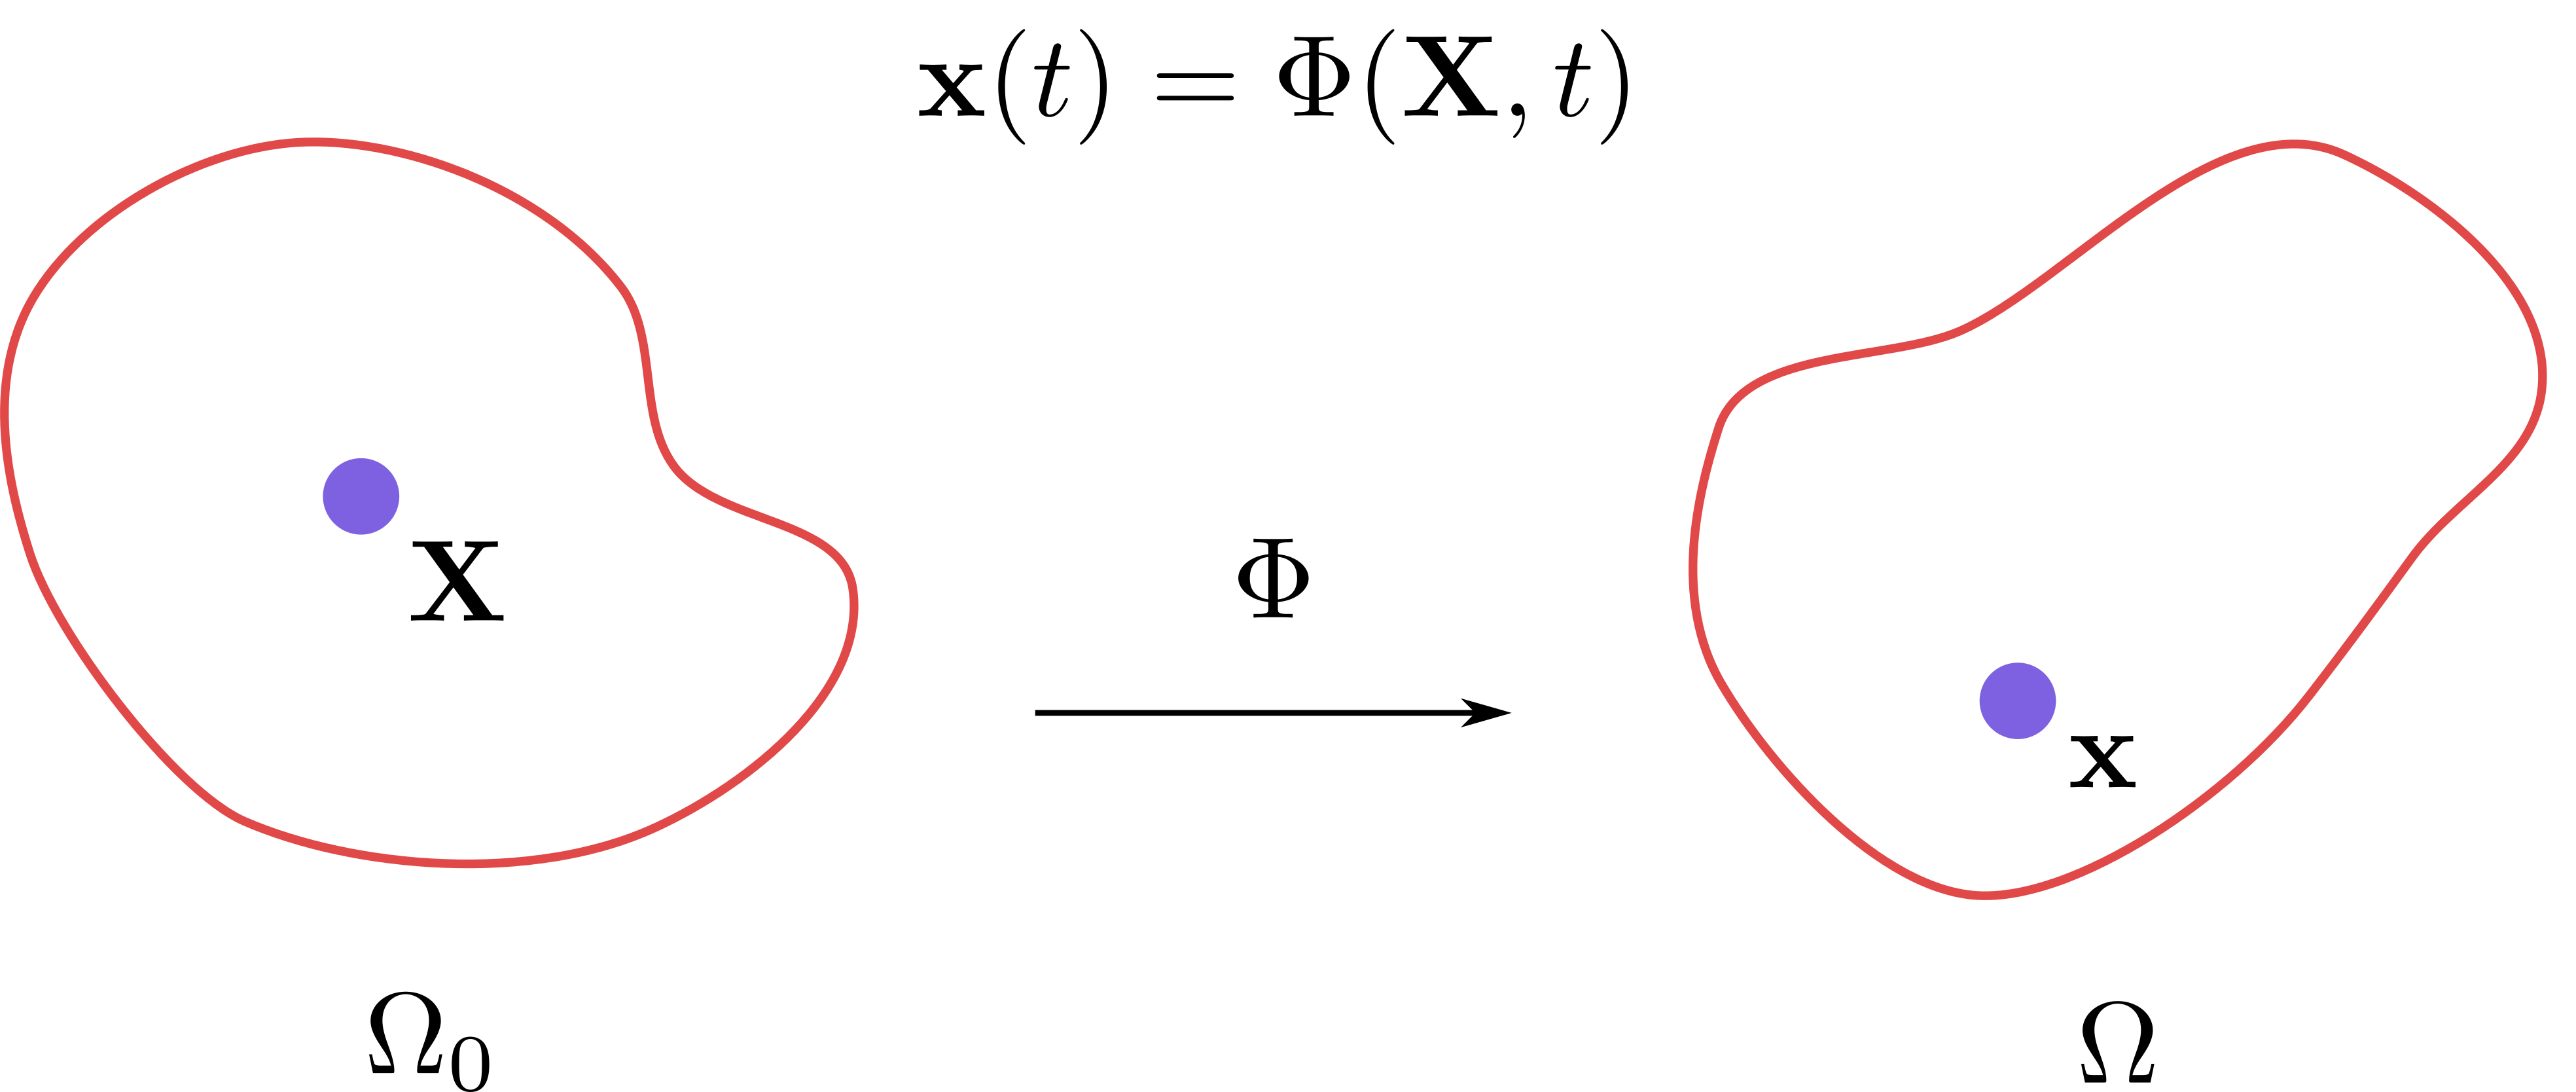
\includegraphics[scale=0.4]{./images/continuum_mechanics/displacementField.png}
\caption[STAR mechanics: Displacement field]{\label{fig:displacementField}
 The displacement field $\Phi$ maps each point $\mathbf{X}$ from the rest configuration $\Omega_{0}$ to a point $\mathbf{x}$ in the deformed configuration $\Omega$.}
\end{figure}
The deformation gradient $F$ describes the local state subject to rigid and/or deformable displacement with respect to the undeformed configuration. It is defined as
\begin{equation}
\label{eq:deformationGradient}
\displaystyle F = \frac{\partial \Phi}{\partial \mathbf{X}}
\end{equation}
The strain tensor $\epsilon$ measures the deformation.
There are many strain measures such as the Green-Lagrange strain
\begin{equation}
\label{eq:greenLagrangeStrain}
\displaystyle \epsilon = \frac{1}{2}\left(F^{T}F - I\right)
\end{equation}
or its linearized version, the Cauchy strain 
\begin{equation}
\label{eq:cauchyStrain}
\displaystyle \epsilon = \frac{1}{2}\left( F + F^{T} \right)-I
\end{equation}
In contrast with the Green-Lagrange strain, the Cauchy strain does not capture well large rotations and therefore is mainly used for small deformations. In Chapter~\ref{chap:cutting}, we use the Green-Lagrange strain for the simulation of elastic thin sheets.
\\
The displacement field, deformation gradient and strain tensor are the main components of the constitutive law that relates the deformation to the material properties of the object.

\subsubsection{Constitutive Law}
For elastic materials, the stress tensor $\sigma$ can be described using constitutive density energy $\Psi$ that is derived with respect to the strain tensor $\epsilon$
\begin{equation}
\label{eq:constitutiveLaw}
\sigma = \frac{\partial \Psi}{\partial \epsilon}
\end{equation}
Different forms of energy exist. 
For an elastic material, also called Hookean material, the density energy is
\begin{equation}
\label{eq:densityEnergy}
\Psi = \frac{1}{2}H\epsilon^{2}
\end{equation}
where $H$ is called the stiffness tensor and is a $3\times3\times3\times3$ tensor. By injecting Equation~\eqref{eq:densityEnergy} into Equation~\eqref{eq:constitutiveLaw}, we get the constitutive law
\begin{equation}
\label{eq:hookeLaw}
\sigma = H\epsilon
\end{equation}
For isotropic materials, the number of material parameters in $H$ can be reduced to two, the Young's modulus $E$ and the Poisson's ratio $\nu$.
These parameters respectively describes the resistance of the object to extension and to shearing.
Moreover, the strain and stress tensor are symmetric which simplifies Equation~\eqref{eq:hookeLaw} to
\begin{equation}
\sigma = 
\begin{bmatrix}
\sigma_{11} \\
\sigma_{22} \\
\sigma_{33} \\
\sigma_{23} \\
\sigma_{13} \\
\sigma_{12}
\end{bmatrix}
=
\tilde{H}
\begin{bmatrix}
\epsilon_{11} \\
\epsilon_{22} \\
\epsilon_{33} \\
2\epsilon_{23} \\
2\epsilon_{13} \\
2\epsilon_{12}
\end{bmatrix}
\end{equation}
where
\begin{equation}
\tilde{H} =
\frac{E}{\left(1+\nu\right)\left(1-2\nu\right)}
\begin{bmatrix}
1-\nu & \nu & \nu & 0 & 0 & 0 \\ 
\nu & 1-\nu & \nu & 0 & 0 & 0 \\
\nu & \nu & 1-\nu & 0 & 0 & 0 \\
0 & 0 & 0 & \frac{1-2\nu}{2} & 0 & 0 \\
0 & 0 & 0 & 0 & \frac{1-2\nu}{2} & 0 \\
0 & 0 & 0 & 0 & 0 & \frac{1-2\nu}{2} \\
\end{bmatrix}
\end{equation}
Instead of computing internal forces as the divergence of the stress, they can be computed as the derivative of the density energy with respect to the degrees of freedom
\begin{equation}
\label{eq:internalForces_solids}
\mathbf{f} = -\int_{\mathcal{V}} \frac{\partial \Psi}{\partial \mathbf{x}}^{T} dv
\end{equation}

\subsubsection{Frame-based model}
\label{subsubsec:framebased}
There are many models to discretize the equations of motion for an elastic solid: Moving Least Squares~\cite{Muller2004:melting}, finite element method~\cite{OBrien1999}, etc.
Here we choose to discretize these equations using the frame-based model, as we will use it in Chapter~\ref{chap:cutting} to handle interactive and detailed cutting of thin elastic objects.
\\
The frame-based model was introduced by Gilles et al.~\cite{Gilles2011} to simulate deformable objects. 
In contrast to other deformable models, it allows to simulate complex object with very few degrees of freedom and to handle heterogeneous materials easily~\cite{Faure2011}. 
Additionally, this work formalized the concept of multi-layer physical framework. 
In the following, we first describe what is a multi-layer framework and illustrate it in the case of the frame-based model. 
Then we detail a standard choice for the different components of the frame-based model: degrees of freedom, interpolation and integration. 
As in the previous section, this section is a high level overview. 
Detailing collision detection and response processes and giving a more accurate formulation of viscosity via the strain rate are out of the scope of this chapter.

\paragraph{A multi-layer physical framework}
Most of the time, the different components of a physics-based model are described as a monolithic framework: degrees of freedom, interpolation, integration and constitutive law are put together in one formula which computes the forces applied on the degrees of freedom. On one hand, this provides a compact and implementation-friendly expression. 
On the other hand, it requires assumptions on each component and make it hard to distinguish what should be changed in order to integrate collisions, to embed a visual model or to test variations of the initial model.

An interesting alternative is to build a multi-layer framework where each component of a physics-based model represents a layer which is able to communicate with other layers through mappings. 
We distinguish three main advantages:
Firstly, the framework has then a great modularity, as different components can be implemented separately, re-used and mixed together. A direct consequence is the ease at prototyping. 
State of the art methods can be implemented in hours instead of days. 
Comparisons of different models is much easier. 
Secondly, as each layer can be discretized at its own resolution, the granularity of the simulation can be easily controlled and computational tasks better distributed.
For instance, in the case of the frame-based model, the sampling of the degrees of freedom is sparse to accelerate the time integration while a denser sampling is used for the integration points in order to accurately compute the deformation.
Finally, embedding techniques, used to display a fine visual model or to handles collision with a coarse representation, fits well in this framework by using the displacement field to map these models to the degrees of freedom.
\\
In their work, Gilles et al.~\cite{Gilles2011} proposed such an alternative by decomposing the computation of force using the derivation chain rule:
\begin{equation}
\label{eq:forceChainRule}
\displaystyle \mathbf{f} = -\int_{V} \left(\frac{\partial \Psi}{\partial \mathbf{x}}\right)^{T} dv
=
-\int_{V} \left(\frac{\partial F}{\partial \mathbf{x}}\right)^{T}
\left(\frac{\partial \epsilon}{\partial F}\right)^{T}
\left(\frac{\partial \Psi}{\partial \epsilon}\right)^{T} dv
\end{equation}
The three different layers are now visible: the degrees of freedom, the deformation gradient, the strain tensor and the constitutive density energy.
Moreover, we can distinguish the Jacobian of the mappings that link degrees of freedom to deformation gradient and deformation gradient to strain.
Notice that the derivative of the constitutive density energy with respect to strain is actually the stress tensor presented in Equation~\eqref{eq:constitutiveLaw}.
In Figure~\ref{fig:multiLayerFramework}, we illustrate this framework in the case of the frame-based model.
\begin{figure}[H]
\centering
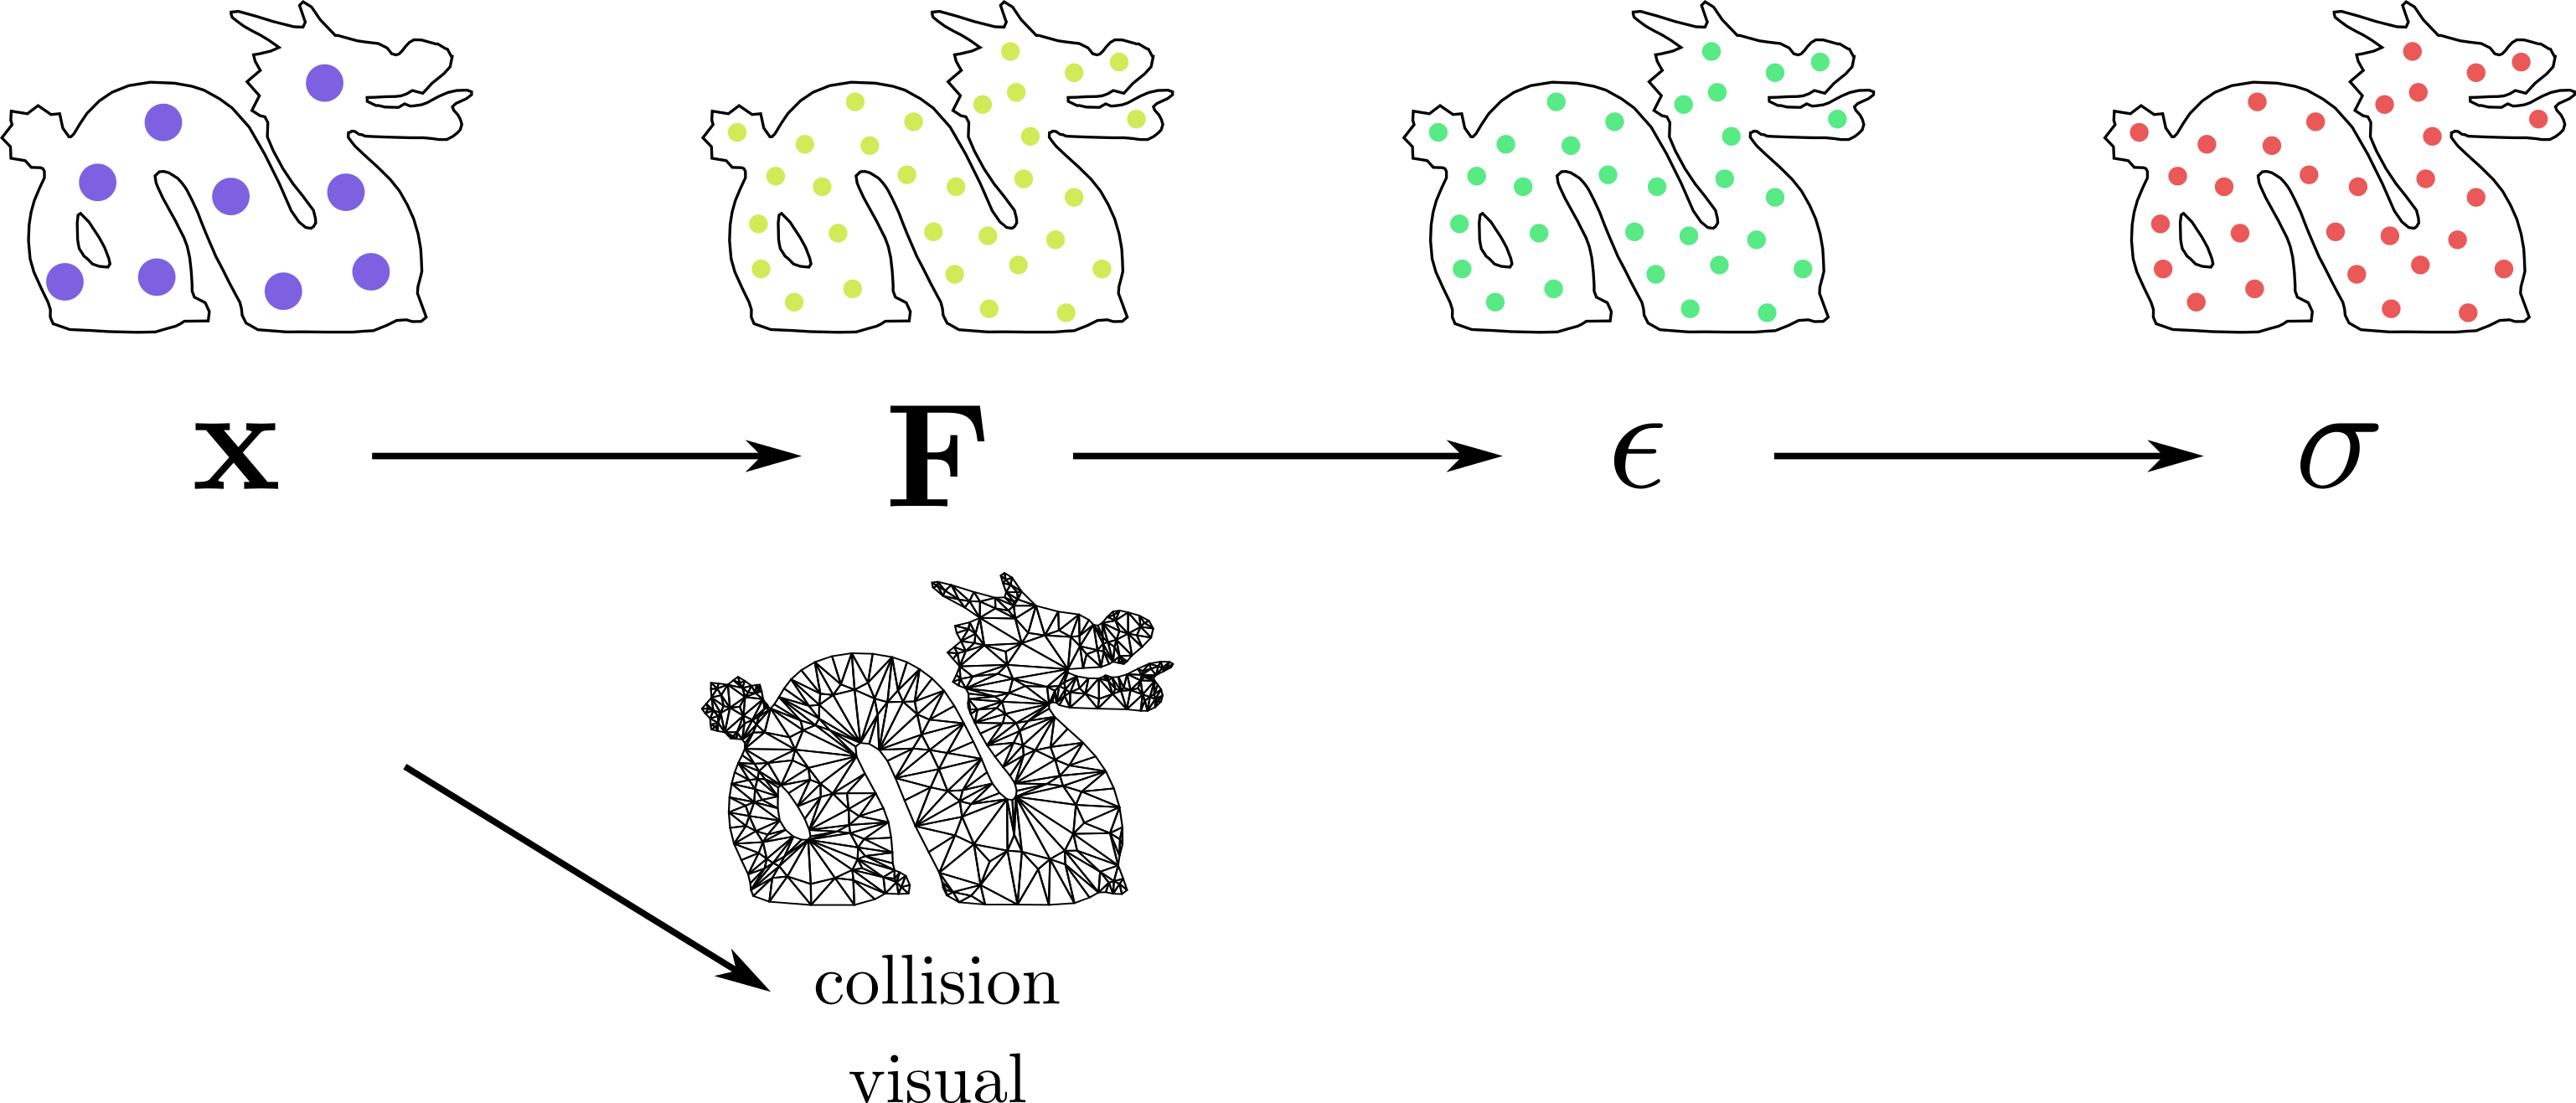
\includegraphics[width=\linewidth]{./images/continuum_mechanics/multiLayeredFramework.png}
\caption[STAR mechanics: Multi-layer framework]{\label{fig:multiLayerFramework} Each component of the simulation is isolated and communicates with other components through mappings. By doing so, the framework allows fast prototyping and comparison of a wide range of deformable models.}
\end{figure}

\paragraph{Degrees of freedom} Let assume that $N$ samples have been uniformly distributed over the object. 
Each sample carries an affine frame $T=(A,\mathbf{t})$ which represents $12$ degrees of freedom: $3$ for translation $\mathbf{t}$, $9$ for the matrix $A$ combining rotation, scaling and shearing. 
Affine frames are expressed with respect to their initial configuration~$T_{0} = \left(A_{0}, \mathbf{t}_{0}\right)$.

\paragraph{Interpolation}
Linear blend skinning is used to interpolate the displacement field and other quantities of the simulation. 
A deformed position $\mathbf{x}$ can be interpolated as a weighted sum of the affine transformations applied to the rest position $\mathbf{x}_{0}$.
\begin{equation}
\label{eq:frameBasedDisplacementField}
\begin{array}{l}
\displaystyle \mathbf{x} = \Phi(\mathbf{x}_{0}) = \sum_{i=0}^{N} w_{i}(\mathbf{x}_{0})\left(\mathbf{t}_{i}+A_{i}\mathbf{x}_{0,i}^{rel}\right) \\ \\
\displaystyle \mathbf{x}_{0,i}^{rel} = A_{0,i}^{-1}\left( \mathbf{x}_{0} - \mathbf{t}_{0,i} \right)
\end{array}
\end{equation}
where 
\begin{itemize}
\item $\mathbf{x}_{0,i}^{rel}$ is the relative position of $\mathbf{x}_{0}$ in the frame defined by $T_{0,i}$.
\item $w_{i}$ is the shape function associated to the frame $i$.
\end{itemize}
Different shape functions can be used. Three properties are important in order to represent a physical behavior. 
First, the shape function should linearly decrease with respect to distance in the material. 
Otherwise, the deformation will not be uniform with respect to the distance from the frame. 
Second, the shape function should be positive. 
Third, the shape functions should form a partition of unity. 
In practice, we use the Voronoi-based shape functions.
In Section~\ref{sec:adaptivesf}, we will detail the computation of Voronoi-based shape functions and how to dynamically update them to take into account topological changes.
\\
From the description of the displacement field (Equation~\eqref{eq:frameBasedDisplacementField}), the deformation gradient can then be derived:
\begin{equation}
\displaystyle
F\left(\mathbf{x}\right) = 
\frac{\partial \mathbf{x}}{\partial \mathbf{x}_{0}} =
\sum_{i=0}^{N} \nabla w_{i}(\mathbf{x}_{0}) \left( \mathbf{t}_{i}+A_{i}\mathbf{x}_{0,i}^{rel}\right) + 
w_{i}\left( A_{i}A_{0,i}^{-1} \right)
\end{equation}

\paragraph{Spatial integration}

Any quadrature rule can be used. Here, for the sake of simplicity, we suppose that we use the midpoint rule (see Equation~\eqref{eq:midpointRule}) briefly described in Figure~\ref{fig:spatialIntegration}.
In contrast with the SPH model that we described in Section~\ref{subsubsec:starSPH}, the sampling of the frames is very sparse.
On one hand this allows to integrate the equations of motion over time very efficiently. 
On the other hand, there are not enough samples to accurately measure the deformation.
To remedy this, an additional denser sampling is used for the integration points.
Let assume that we sampled the object with $M$ integration points, then we can use the midpoint rule to compute the internal forces for one frame as
\begin{equation}
\label{eq:frameForceComputation}
\displaystyle
\mathbf{f}_{i} =
- \sum_{j=0}^{M}
\left( \frac{\partial F}{\partial \mathbf{x}_{i}} \right)^{T}
\left( \frac{\partial \epsilon}{\partial F} \right)^{T}
\left( \frac{\partial \Psi}{\partial \epsilon} \right)^{T} \left(\mathbf{x}_{j}\right) V_{j} 
\end{equation}
where 
\begin{itemize}
\item $\mathbf{x}_{j}$ is the position of the integration point $j$.
\item $V_{j}$ is volume associated to integration point $j$.
\end{itemize}

\paragraph{Temporal integration}
Assuming the mass matrix is lumped and that we use symplectic Euler, the time integration of one frame $i$ is:
\begin{equation}
\displaystyle
\begin{array}{l}
\begin{pmatrix}
\mathbf{t'}_{i}(_{n+1}) \\
A'_{i}(t_{n+1})
\end{pmatrix} 
=
\begin{pmatrix}
\mathbf{t'}_{i}(t_{n}) \\
A'_{i}(t_{n})
\end{pmatrix} 
+
\Delta t
M_{i}^{-1}
\left(\mathbf{f}_{i}(t_{n}) + M_{i}\mathbf{g} \right)
\\ \\
\begin{pmatrix}
\mathbf{t}_{i}(_{n+1}) \\
A_{i}(t_{n+1})
\end{pmatrix} 
=
\begin{pmatrix}
\mathbf{t}_{i}(t_{n}) \\
A_{i}(t_{n})
\end{pmatrix} 
+
\Delta t
\begin{pmatrix}
\mathbf{t'}_{i}(_{n+1}) \\ A'_{i}(t_{n+1})
\end{pmatrix} 
\end{array}
\end{equation}
where $M_{i}$ is the mass matrix of the frame $i$:
\begin{equation}
\label{eq:massMatrix}
M_{i} = \int_{V} w_{i}^{T} \rho w_{i} dv
\end{equation}
and $\rho$ is the density of the object.
\\ \\
We described the key ingredients to simulate elastic solids using the frame-based model.
As for fluid mechanics, there are many other related topics that we choose not to detail here.
For the formulation of implicit Euler and a survey of collision detection techniques, we respectively refer the reader to the course of Witkin et al.~\cite{Witkin2001} and the work of Teschner et al.~\cite{Teschner2005}.

\subsection{Conclusion on continuum mechanics}
In this section, we briefly presented the basics of continuum mechanics.
First, we described how to design equations of motion and which numerical tools are involved in their solving. 
Then, for fluids and solids mechanics, we mentioned their specificities and detailed a deformable model.
We illustrated the fact that continuum mechanics allows to automatically compute realistic motion from a wide range of phenomena.
This strength mainly explains why hand-made animations of physical phenomena have been replaced by physics-based animation.
However, realism comes with a high computational cost which can make large scale simulations intractable or can prevent from simulating advanced phenomena in interactive context.
In the following section, we review adaptive models, a common approach to make simulations efficient.
